\documentclass{report}
\usepackage{amsmath}
\usepackage{ dsfont }
\usepackage{ svg }

\usepackage[colorlinks,citecolor=black,linkcolor=black,urlcolor=blue,bookmarks=false,hypertexnames=true]{hyperref}\usepackage{kpfonts}
\usepackage[T1]{fontenc}
\usepackage{nimbusmononarrow}
\usepackage[utf8]{inputenc}
\usepackage{graphicx}
\usepackage{subfigure}
\usepackage{caption}
\usepackage{titling}
  \usepackage{float}
  \usepackage{textcomp}
\begin{document}


\pretitle{%
  \begin{center}
  \LARGE
  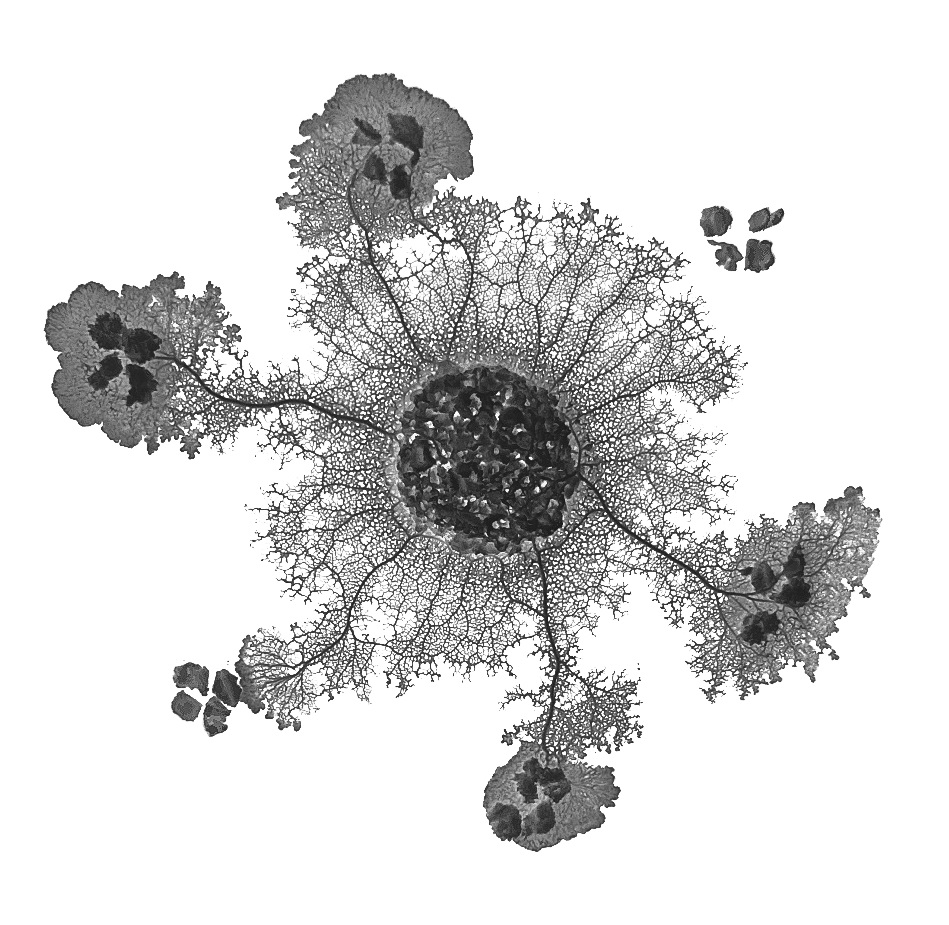
\includegraphics[height=10cm]{final_lightroom_inverted.jpg}\\[\bigskipamount]
}

\title{%
  \Huge Physarum\\
  \large Slime mould computing simulation\\
    }
\author{
  Coppola Matteo\\
  \texttt{793329}
  \and
  Palazzi Luca\\
  \texttt{793556}
   \and
  Vivace Antonio\\
  \texttt{793509}
}
\date{Complex Systems: Models and Simulation, \\ September 2019}
\maketitle

\begin{abstract}
We introduce and define the Cellular Automata mathematical model, used to describe the evolution of discrete systems. We give an overview of its relevancy and applications in different fields.

We use this tool to model the "intelligent" behavior of \textit{Physarum polycephalum}, a slime mould extensively studied for its interesting characteristics:

Despite the protist not having a nervous system, it has the capacity to solve computational challenges such as the Shortest Path and instances of the Transportation Problem.
It also exhibits a form of memory and creates efficient networks when given more than two food sources, being able to dynamically re-allocate itself to maintain constant levels of different nutrients simultaneously.

Our main work has been creating an improved Physarum model that performs more similarly to the real mould than the current proposed approximations offered by the scientific community.
Our experimental model closely follows the real mould behaviour without violating the Celluar Automata definition, returning interesting results often more realistic than the other public models.
We proceed to study the global behaviour and topologies that raise from our Cellular Automata rules, applying the simulation on several maps and finally discussing the results and the possible improvements.

We proceed to build a cross-platform software framework to run and visualize a simulation of the described model using modern tools. A UI exposes a series of control features, letting the user monitor and control the simulation.

\end{abstract}
\addtocounter{page}{-1}
\tableofcontents
\listoffigures

\section{Cellular Automata}
\label{automi_cellulari}

A Cellular Automaton (abbrev. CA) is a discrete and dynamic mathematical model capable of storing and processing information on a set of rules.
\par
The basic idea of CAs is the simulation of complex behaviors deriving from natural systems.
\par
The concept was originally described and defined in the 1940s by Stanislaw Ulam and John von Neumann, who use them to simulate natural and biological processes. The interesting part of this process is not only the simulation as an imitation of biological behaviors, but the creation of automatic models that can investigate the true nature of complex systems existing in nature. In this way, cellular automata become a tool to study self-organization and emergence in complex systems.
\par
A CA consists of a regular grid of cellss. Each cell can take a finite number \texttt{k} of different states, where \texttt{k} is a number equal or greater than 2. Cells update their states in discrete time. The time step t = 0 is usually considered as the initial step and a given state is assigned to each cell: the set of these states constitutes the initial configuration of the cellular automaton.
At each time step (usually advancing t of 1) each cell is updated and following the invariant over time system's rules a new generation replaces the previous generation. The state change of each single cell is determined only by its current status and by the states of the cells close to the current one.
\par
Regarding the two-dimensional CAs, there are two fundamental types of neighbourhoods that are mainly considered:
\begin{itemize}
\item von Neumann neighbourhood, that consists of the central cell, whose condition is to be updated, and the four cells located to the north, south, east and west of the central cell
\item Moore neighbourhood, that consists of the same cells with the von Neumann neighbourhood together with the four other adjacent cells of the central cell (the north-west, north-east, south-east and south-west cells)
\end{itemize}
\par
The most known CA in the scientific literature is \texttt{the Game of Life}, devised by the John Horton Conway in 1970 with the intention of producing a simple model of von Neumann's idea of the machine capable of reproducing itself and simulate a Turing machine. 
\par
In the universe of \texttt{the Game of Life} each cell is in one of two possible states, alive or dead (or populated and unpopulated, respectively). Every cell interacts with its eight neighbours, which are the cells that are horizontally, vertically, or diagonally adjacent. At each step in time, the following transitions occur:
\begin{itemize}
\item Any live cell with fewer than two live neighbours dies, as if by underpopulation
\item Any live cell with two or three live neighbours lives on to the next generation
\item Any live cell with more than three live neighbours dies, as if by overpopulation
\item Any dead cell with exactly three live neighbours becomes a live cell, as if by reproduction
\end{itemize}
\par
The initial pattern constitutes the seed of the system. The first generation is created by applying the above rules simultaneously to every cell in the seed; births and deaths occur simultaneously, and the discrete moment at which this happens is sometimes called a tick. Each generation is a pure function of the preceding one. The rules continue to be applied repeatedly to create further generations. 

\section{Physarum}

Physarum polycephalum\cite{Tsompanas2016} is a species of order Physarales, subclass Myxogas-tromycetidae, class Myxomecetes, division Myxostelida, commonly known as a true slime mold, that inhabits shady, cool and moist areas. 
\par
Physarum thrives in favorable environmental conditions, particularly when the right combinations of humidity, temperature and nutrient presence are created. If the conditions are not adequate for development, Physarum behaves like a single-celled organism that does not demonstrate organizational skills. In appropriate conditions, it joins together to create particularly efficient filamentary nets in physical distribution.
\subsection{Life cycle}
For most of the life cycle Physarum is found in the form of a single cytoplasmic mass, called plasmodium, a plurinuclear cell made up of networks of protoplasmic veins that can contain more than 100,000 nuclei. It is during this stage that the organism searches for food. The plasmodium surrounds its food and secretes enzymes to digest it.
\par
If environmental conditions cause the plasmodium to desiccate during feeding or migration, Physarum will form a sclerotium. The sclerotium is basically hardened multinucleated tissue that serves as a dormant stage, protecting Physarum for long periods of time. Once favorable conditions resume, the plasmodium reappears to continue its quest for food.
\par
As the food supply runs out, the plasmodium stops feeding and begins its reproductive phase. Stalks of sporangia form from the plasmodium. It is within these structures that meiosis occurs and spores are formed. Sporangia are usually formed in the open so that the spores they release will be spread by wind currents.
\par
Spores can remain dormant for years if need be. However, when environmental conditions are favorable for growth, the spores germinate and release either flagellated or amoeboid swarm cells (motile stage). The swarm cells then fuse together to form a new plasmodium. 
\subsection{State of the art}
An increasing number of researchers have conducted studies concerning the Physarum to explore its intelligence in the field of optimal problems. This happened due to some biological experiments observed in laboratory conditions in which the Physarum exhibited extraordinary capacities to build efficient networks.
A first example to analyze is the work of Nakagaki et al. in 2000 (T. Nakagaki, H. Yamada, and A. Toth, “Intelligence: Maze-solving by an amoeboid organism,”). In this experiment Physarum show his intelligent behavior successfully found the shortest path between two selected points in a maze. In another famous experiment\cite{Tero439} operated by Tero et al. in 2010, Physarum built networks with comparable qualities to those of Tokyo rail system.
\par
In the recent years, computer scientists have been inspired by biological systems for computational approaches, in particularly with respect to complex optimization and decision problems\cite{Grube2016PhysarumQV}. In this context, Physarum emerged as a model organism which has attracted substantial interest.  The aforementioned experiments require expensive and specialized equipment and some experience on basic biological laboratory techniques. However, the majority of scientists are unfamiliar with such methods. 
\par
A commonly proposed alternative alleviating these difficulties is software models that simulate the behavior of the plasmodium and provide similar results. The advantages of a software model over the real Physarum are repeatability and faster productions of results.
\par
As slime mould has no brain or any central processing system, its distributed control can be perfectly described by the local rule of CAs. It is noteworthy that CAs are known for emerging global behavior from local interactions. The CA model was firstly proposed by Gunji et al. in 2008 to design high-quality networks. In this model, the optimization process is consistent with the properties of real cells. 

\chapter{State of the Art}
An increasing number of researchers have conducted studies concerning the Physarum to explore its intelligence in the field of optimal problems. This happened due to some biological experiments observed in laboratory conditions in which the Physarum exhibited complex patterning, adaptive behavior and extraordinary capacities to build efficient networks.
\par
It is very important to remember that the slime mould is a puzzling organism because it possesses no neural tissue yet, despite this, are known to exhibit complex biological and computational behavior: it is not explicitly trying to solve computational problems. So the idea served by several researchers was how to take advantage of Physarum’s to survive in order to solve complex problems. 

\section{Biological approach}
In the laboratory experiments that demonstrate these computing capabilities, small food sources - agar blocks containing ordinary oat flakes - are presented at various positions to a starved plasmodium, it endeavours to reach them all; as a consequence, only a few tubes are in contact with each individual food source.  The organism attempts to optimize the shape of the network to facilitate effective absorption of the available nutrients. However, this might be difficult to achieve when multiple food sources are presented because of the limited body mass of the organism.
\par
This network shape of the body enables certain physiological requirements to be met \cite{nakagaki2004obtaining}:
\begin{itemize}
	\item absorption of nutrients from food souces as efficiently as possible because almost all the body mass stays at the food sources to enable absorption
	\item maintenance of the connectivity and intracellular communication throughout the organism
	\item meeting the constraint of limited resource of body mass. The network shape is regarded as a solution for the
organism’s survival problems.
\end{itemize}

Contrary to this, if food is plentiful, the organism finally splits into two pieces on two food sources.

\par
The organism requires a well hydrated substrate. All true slime moulds reproduce by sporulation. Certain factors, such as starvation, light irradiation and dehydration will prompt the plasmodium to irreversibly transform into a multitude of black, globulose structures known as sporangia that harbour the organism’s spores.
\par
The name Physarum refers to the fact that multiple apparently autonomous leading edges may exist in one plasmodium. This is an observation of note as some of the first work on slime mould was based on the principle that Physarum can "choose" the most efficient path between food sources.

\subsection{Biological experiments}
The biological basis for this involves the Physarum identifying chemical gradients with multiple advancing margins before deciding to navigate along the strongest gradient. This has been interpreted as slime mould undertaking problem solving and network optimization, such as demonstrated in the following ground-breaking experiments.

\paragraph{Maze solving}
Nakagaki et al. \cite{nakagaki2000intelligence} were the first to observe that the plasmodium of the slime mould changes its shape as it crawls over a plain agar gel. If food is placed in two certain spots, it puts out pseudopodia that connect those food spots. The most interesting part is that the plasmodium had the ability to find the minimum-length solution between two points in a maze. This happens because Physarum reduces its mass, from the paths of the maze that is far from the minimum distance, and strengthens its tubes that belong to the minimum distance.

\paragraph{Network formation}
In 2010 Tero et al. \cite{Tero439} compared the actual rail network in Japan with a Physarum network consisted by 36 nutrients sources (NSs) that represented the geographical locations of cities in Tokyo area. The Physarum was planted on Tokyo and from there started its foraging  and exploration for NSs until it filled much of the available land space. Then the organism started to concentrate on the NSs by thinning out the network to leave a subset of larger interconnecting tubes. The topology of many Physarum networks appeared similar to the rail network. The conclusion was that Physarum networks showed characteristics with comparable qualities to those of the rail network in terms of cost, transport efficiency and fault tolerance.\\

\par
AGGIUNGERE MODELLO MATEMATICO?
\par

\par
SEZIONE SEPARATA?

\section{CS approach}
In the recent years, computer scientists have been inspired by biological systems for computational approaches, in particularly with respect to complex optimization and decision problems \cite{grube2016physarum}. In this context, Physarum emerged as a model organism which has attracted substantial interest. The aforementioned experiments require expensive and specialized equipment and some experience on basic biological laboratory techniques. However, the majority of scientists are unfamiliar with such methods and the experiments on a living organism may last a lot of hours or maybe some days to provide data.
\par
A commonly proposed alternative alleviating these difficulties is software models that simulate the behavior of the plasmodium and provide similar results. The advantages of a software model over the real slime mould are repeatability and faster productions of results.
\par
As slime mould has no brain or any central processing system, its distributed control can be perfectly described by the local rule of CAs. It is noteworthy that CAs are known for emerging global behavior from local interactions. 
\par
Consider only the plasmodium stage of its life cycle, there is no single model that can describe exactly the behavior of Physarum. So far, there is a variety of modeling approaches which also are implemented by a variety of tools \cite{Tsompanas2016}, \cite{gunji2008minimal}, \cite{shirakawa2015construction}.
\par
All of the biological studies indicated above, like solving a maze and designing a transport network, have observed the optimization behaviour of the plasmodium with the experimental setups roughly consisting of three steps \cite{shirakawa2015construction}:
\begin{itemize}
	\item First step: the plasmodium fully searches the given space
	\item Second step: some sources of attractant or repellent stimuli are given to the plasmodium that is fully and homogeneously spreading in the space
	\item Third step: the plasmodium optimizes the connection between the sources
\end{itemize}

The majority of the studies focus on the behaviour of the plasmodium in a closed space. However, few studies have been done for the plasmodium that is exploring an open space. 
\par
INIZIO CONSIDERAZIONI
\par
We believe that we can find more enhanced biological characteristics of the biological entities by observing the behaviours of them in an open and unknown environment. In this study, we thus tried to investigate the exploratory behaviour of the plasmodium in an open space and to understand how the organism makes its decision in exploration. 
\par
FINE CONSIDERAZIONI



\chapter{Model}
In this project the behaviour of slime mould during the laboratory experiments have been simulated using models based on Cellular Automata. Using CA can be justified by the emergence of global behaviour from local interactions, a rule that applies also on the real slime mould.

\section{Paper model}

After reviewing the literature on several models, we have decided to use the CA based model of Tsompanas et al. \cite{Tsompanas2016} that mimics the foraging strategy and tubular network formation. In particular, the model is based on the representation of diffusion of chemical attractants by NSs and the attraction of the plasmodium, which initiates its exploration from the starting point (SP), by these chemicals. 

\par
The plasmodium is first starved and then introduced to an exploring region in a SP. Moreover, some NSs which produces chemo-attractants are located at characteristic points. 

\par
The plasmodium starts searching for nutrients, exhibiting pattern of guided movement towards/away from sources of stimulation; it explores the available area, encapsulates the NSs and creates a tubular network that connects all these NSs by a nature-inspired, cost effective and risk avoiding manner.
Typically, slime mould is stimulated in experimental situations by providing a number of spatially distributed chemoattractant nutrient NSs towards which it will migrate (chemotaxis).

\par
To note the geometry of the network created by the plasmodium depends on the positions of the NSs. Moreover, further parameters can play key role in determining exact structure of plasmodium network.

\par
In order to imitate and simulate a biological laboratory experiment, the entire area is divided into a matrix of squares with identical areas - that constitutes a set defined as E - and each square of the surface is represented by a CA cell.
This area can be categorized as available area (a set of cells defined as A) and unavailable area (a set of cells defined as U) for the development of the plasmodium.
Also some cells that are included in the available area set of cells, represent the oat flakes that are considered as NSs for the plasmodium (a set of cells defined as N) and one cell represents the place where the plasmodium is initially introduced to the
experimental environment or the SP (a set of one cell defined as S).
The neighbourhood type used for the model is Moore neighbourhood and the state of the $c_{(i, j)}$ cell at time step t ($ ST^t_{(i, j)}$) is defined as:
\begin{align}
ST^t_{(i, j)} = [AA_{(i, j)}, PM^t_{(i, j)}, CHA^t_{(i, j)}, TE^t_{(i, j)}]
\end{align}
where:

\begin{itemize}
	\item $AA$ stands for Available Area for the exploration by the plasmodium. It assumes a boolean value:  	
\[AA_{(i, j)}=\begin{cases} \mbox{True}, & \forall i, j: c_{(i,j)} \in A \\ \mbox{False}, &  \forall i, j: c_{(i,j)} \in U\end{cases}\]
	\item $PM$ (Physarum Mass) is a floating-point variable. It indicates the volume of the cytoplasmic material of the plasmodium located on a specific cell. This parameter can have any value in the continuous space of [0–100]
	\item $CHA$ (CHemoAttractant) is a floating-point variable. It represent the concentration of chemo-attractants that are located on a specific cell. This parameter can have any value in the continuous space of [0–100]
	\item $TE$ stands for Tube Existence and represents the participation of a cell in the tubular network inside the body of the slime mould
\end{itemize}

The initial values for parameters $PM$ and $CHA$ are defined as:
\begin{align}
PM^t_{(i, j)}=\begin{cases} 100, & \forall i, j: c_{(i,j)} \in S \\ 0, & \mbox{else}\end{cases}
\end{align}
\begin{align}
CHA^t_{(i, j)}=\begin{cases} 100, & \forall i, j: c_{(i,j)} \in N \\ 0, & \mbox{else}\end{cases}
\end{align}

Taking into consideration the assumptions made for the way the Physarum develops through an available area, which were confirmed by laboratory experiments, it is determined that the plasmodium is "amplified" at a NS and then searches for other NSs, considering the recently encapsulated NS as a new SP. Also, when a NS is covered by the plasmodium, the generation of chemoattractant substances is ceased.
In the model the NSs are turned into SPs when the plasmodium encapsulates them with a sufficient amount of mass. Furthermore, it is realized that the plasmodium is propagating away from the most recently captured NS by taking a semi-circular form. 

\par
The initialization step includes the definition of parameters that have a great impact on the results of the model. These parameters include:
\begin{itemize}
	\item The length of the CA grid
	\item The parameters for the diffusion equation for the cytoplasm of the plasmodium (PMP1, PMP2)
	\item The parameters for the diffusion equation of the chemo-attractants substances (CAP1, CAP2)
	\item The consumption percentage of the chemo-attractants substances by the plasmodium (CON - Consumption)
	\item The attraction of the slime mould by chemoattractant substances (PA - Physarum Attraction)
	\item The threshold of Physarum Mass that encapsulates a NS (ThPM).
\end{itemize}

\par
After the initialization and for 50 time steps, diffusion equations are used to calculate the values for $CHA$ and $PM$ for every cell in the grid. Every cell uses the values of its neighbours at time step t to calculate the value of the $CHA$ and $PM$ parameter for time step t + 1. 

\par
The contribution to the diffusion of the Physarum Mass of the von Neumann neighbours ($PMvNN$) of the $c_{(i,j)}$ cell is defined as:
\begin{equation}
\begin{split}
PMvNN^t_{(i, j)} = 
(1 + PA^t_{(i, j),(i-1, j}) \times PM^t_{(i-1, j)} - AA_{(i-1, j)} \times PM^t_{(i, j)} +
\\(1 + PA^t_{(i, j),(i, j-1}) \times PM^t_{(i, j-1)} - AA_{(i, j-1)} \times PM^t_{(i, j)} +
\\(1 + PA^t_{(i, j),(i+1, j}) \times PM^t_{(i+1, j)} - AA_{(i+1, j)} \times PM^t_{(i, j)}  +
\\(1 + PA^t_{(i, j),(i, j+1}) \times PM^t_{(i, j+1)} - AA_{(i, j+1)} \times PM^t_{(i, j)}
\end{split}
\end{equation}
Moreover, the contribution to the diffusion of the Physarum Mass of the exclusively Moore neighbours ($PMeMN$) of the $c_{(i,j)}$ cell is defined as:
\begin{equation}
\begin{split}
PMeMN^t_{(i, j)} = 
(1 + PA^t_{(i, j),(i-1, j-1}) \times PM^t_{(i-1, j-1)} - AA_{(i-1, j-1)} \times PM^t_{(i, j)} +
\\(1 + PA^t_{(i, j),(i+1, j-1}) \times PM^t_{(i+1, j-1)} - AA_{(i+1, j-1)} \times PM^t_{(i, j)} +
\\(1 + PA^t_{(i, j),(i-1, j+1}) \times PM^t_{(i-1, j+1)} - AA_{(i-1, j+1)} \times PM^t_{(i, j)}  +
\\(1 + PA^t_{(i, j),(i+1, j+1}) \times PM^t_{(i+1, j+1)} - AA_{(i+1, j+1)} \times PM^t_{(i, j)}
\end{split}
\end{equation}

The total $PM$ for a cell $c_{(i,j)}$ for time t + 1 is a sum of the contributions of its neighbours with appropriate weights and is defined as:
\begin{equation}
PM^{t+1}_{(i, j)} = PM^t_{(i, j)} + PMP1 \times [PMvNN^t_{(i, j)} + PMP2 \times PMeMN^t_{(i, j)}]
\end{equation}
The equation represents the exploration of the available space by the plasmodium which is affected by chemoattractants. The values PMP1 and PMP2 depict that the von Neumann and the exclusively Moore neighbours have different contributions on the diffusion of these parameters. If a neighbouring cell is representing unavailable area, there is no contribution to the diffusion.
 
\par
The parameter $PA_{(i, j),(k,l)}$ represents the attraction of the plasmodium - in cell $c_{(i,j)}$ - by the chemo-attractants towards the direction of an adjacent cell $c_{(k,l)}$, modeling the attraction of the organism towards the higher gradient of chemoattractants. It is equal to a predefined constant (PAP) for the neighbour with the higher concentration of chemo-attractants and equals to the negative value of the parameter PAP for the neighbour across the neighbour with the higher value of chemoattractant, in order to simulate the non-uniform foraging behavior of the plasmodium. For the other neighbours in an area that has no chemo-attractants, then the foraging strategy of the plasmodium is uniform and these parameters are equal to zero.

\par
The $PA$ parameter for cell $c_{(i,j)}$ towards its north neighbour $c_{(i-1,j)}$ is defined as:
\begin{equation}
PA^t_{(i, j),(k,l)}=
\begin{cases} 
PAP, & if CHA_{(i-1, j)} = MAX(CHA_{(k, l)} \forall k, l: i - 1 \leq k \leq i + 1 \\and j - 1 \leq l \leq j+1) \\ 
- PAP, & if CHA_{(i-1, j)} = MAX(CHA_{(k, l)} \forall k, l: i - 1 \leq k \leq i + 1 \\and j - 1 \leq l \leq j+1) \\ 
0, & \mbox{else}
\end{cases}
\end{equation}

\par
The contribution to the diffusion of the chemoattractants for the plasmodium of the von Neumann neighbours ($CHAvNN$) of the $c_{(i,j)}$) cell is defined as:
\begin{equation}
\begin{split}
CHAvNN^t_{(i, j)} = 
(CHA^t_{(i-1, j)}) - AA_{(i-1, j)} \times CHA^t_{(i, j)} +
\\(CHA^t_{(i, j-1)}) - AA_{(i, j-1)} \times CHA^t_{(i, j)} +
\\(CHA^t_{(i+1, j)}) - AA_{(i+1, j)} \times CHA^t_{(i, j)}  +
\\(CHA^t_{(i, j+1)} - AA_{(i, j+1)} \times CHA^t_{(i, j)}
\end{split}
\end{equation}

Moreover, the contribution to the diffusion of the chemoattractants for the plasmodium of the exclusively Moore neighbours ($CHAeMN$) of the $c_{(i,j)}$ cell is defined as:

\begin{equation}
\begin{split}
CHAeMN^t_{(i, j)} = 
(CHA^t_{(i-1, j-1)}) - AA_{(i-1, j-1)} \times CHA^t_{(i, j)} +
\\(CHA^t_{(i+1, j-1)}) - AA_{(i+1, j-1)} \times CHA^t_{(i, j)} +
\\(CHA^t_{(i-1, j+1)}) - AA_{(i-1, j+1)} \times CHA^t_{(i, j)}  +
\\(CHA^t_{(i+1, j+1)}) - AA_{(i+1, j+1)} \times PM^t_{(i, j)}
\end{split}
\end{equation}

As a result, the total $CHA$ for a $c_{(i,j)}$ cell for time t + 1 is defined as:
\begin{equation}
CHA^{t+1}_{(i, j)} = CON \times {CHA^t_{(i, j)} + CAP1 \times (CHAvNN^t_{(i, j)} + CAP \times CHAeMN^t_{(i, j)})}
\end{equation}
The equation represents the diffusion of chemoattractants from the NSs in the available space. The values CAP1 and CAP2 depict that the von Neumann and the exclusively Moore neighbours have different contributions on the diffusion of these parameters. The multiplication with the parameter CON provides the imitation of the consumption of the chemoattractant substances by the plasmodium. Also in this case as in the diffusion of $PM$, if a neighbouring cell is representing unavailable area there is no contribution to the diffusion.

\par
After every 50 time steps of calculating the diffusion equations in the available area, the operation of designing the tubular network takes place. If any NS is covered with over the predefined PM (ThPM), each NS cell is connected to a SP cell by a tubular path from the NS cell to the SP cell, following the increasing gradient of parameter PM of neighboring cells. 
More specifically, starting from the cell representing the encapsulated NS, the adjacent cell with the higher PM value is selected to participate to the tubular network. Then the cell selected to participate to the tubular network selects the next cell from its neighbours with the higher PM value to participate to the tubular network and so on, until a SP is reached.

\par
Finally, the NS cell is transformed to a SP, which means changing its parameters as illustrated in the following equations:

\begin{equation}
PM^t_{(i, j),(k,l)}=
\begin{cases} 
0, & \forall i, j: c_{(i,j)} \in U \\ 
100, & \forall i, j: c_{(i,j)} \in S \\ 
100, & \forall i, j: c_{(i,j)} \in N and  PM^t_{(i, j)} \geq ThPM 
\end{cases}
\end{equation}

\begin{align}
CHA^t_{(i, j),(k,l)}=
\begin{cases} 
100, & \forall i, j: c_{(i,j)} \in N and PM^t_{(i, j)} < ThPM\\ 
0, & \forall i, j: c_{(i,j)} \in N and  PM^t_{(i, j)} \geq ThPM 
\end{cases}
\end{align}

If more NSs are covered with the ThPM, each is connected to the nearest SP and they are all transformed to SPs. 

\section{Experimental model}

The model introduced in the previous section considers only slime mould foraging behaviour and also - with the only information in the paper - seems not to follow the true behavior of slime mould. For this reason we have proposed our new experimental model based on that of Tsompanas et al. \cite{Tsompanas2016}, which objective was to fix the issues that emerged from the many executions of the original model, in particular regarding the calculation of $PM$ and other related aspects.

\subsection{Improvements}
Their algorithm reaches the results for the different types of simulation neglecting important realistic constraints such as mass conservation, resulting in topologies that sometimes slightly differed from the Physarum's. We found their CA's behaviour an excessive approximation of the real mould dynamics, therefore we worked on improving their original algorithm to the point of changing most of the steps.

\par
To accomplish this task, we went back observing the actual behaviour of Physarum. From all the scientific evidence, the first thing we noted was that the mould had a finite amount of mass that it could use to expand and explore the sorroundings. Only when a N was digested more mass was created. 

\par
Our model quantizes the mass and sets a discrete starting amount of mass that is placed on the SP at the beginning of the simulation. This amount must be enough to reach the various NSs placed in the map, otherwise the expansion will simply stop. In reality, when the Physarum can't reach any NSs it simply contracts and eventually goes into another phase of its life cycle.

\par
If no external stymolus is given to the virtual mould, it expands uniformly in all directions to find clues (the chemoattractant) about reachable NSs until it runs out of available mass. As in Tsompanas et al. \cite{Tsompanas2016}, every NS releases chemoattractant in an uniform way around the available area of the map. Therefore after some ticks each free cell of the map contains some chemottractant, creating a gradient that conducts to the NSs.

\par
As soon as the mould finds one of these cells, it stops the uniform expansions and starts moving the whole mass to follow the gradient. This can happen in more than a location at the same time moving the available mass in many directions depending on the number of near NS, exactly how the real Physarum behaves.

\par
During the uniform expansion each neighbour cell that has a lower amount of mass ($PM$) receives some, moving the mass from a nearby cell thus conserving the total amount of mass. If a cell has PM lower than a threshold value, it can't distribute its mass to its neighbours. This local rule generates the typical circular explorative behaviour of the mold.

\par 
When there is a chemoattractant gradient, the mass is moved to the cells that have a higher $CHA$, except if the cell mass is lower than the same previous threshold. This rule causes the elongation of the mould towards the NSs.

\par
Once an NS is reached, more and more mass is accumulated on that cell until it reaches a threshold value as in Tsompanas et al. \cite{Tsompanas2016}. At this point the tube formation process begins.

\par
As the many biological studies about Physarum show, the mould's plasmodium contains fibers that get an orientation based on the vector of expansion. The more the mould is stretched the more these fibers align perfectly into the direction of the stretch. When it finally reaches an NS, all the fibers are already correctly aligned from the SP to the reached NS. The mould then shrinks around the shortest path between NS and SP, condensating the oriented fibers forming the visible tubes that will transport the nutrients towards SP.

\par
Tsompanas et al. \cite{Tsompanas2016} creates the tubes out of nothing as if they are artifacts assembled by the Physarum on the fly. This is wrong as the tubes are a simply result of condensed fibers along the best path. Our model assigns to each available cell a new variable containing the "direction of stretch": when the cell receives some mass for the first time it remembers the direction of the neighbour with the highest PM. The resulting gradient simulates the alignment of the fibers.

\par
When the nearest NS is reached with enough mass the gradient is followed backward to enstablish the shape of the tube, then the NS is changed into a new SP with a new amount of available mass and its CHA value is set to zero as the nutrient has been correctly digested.

\par
At this step the best path has been enstablished but the tubes are not yet visible because the mould mass is still distribuited in all the cells with high $CHA$ gradient.
As Tsompanas et al. \cite{Tsompanas2016} create the tubes on the fly, they don't pay attention to and haven't coded this typical Physarum step: the shrinking process.

\par
During the laboratory experiments after a while the mould shrinks to optimize the usage of its mass, condensing it around the tubes and the SPs, eventually showing the famous network topology.
To correctly simulate this behaviour in our model, every cell that contains some mass gets older at every tick of the simulation. When the age of a cell that is not part of a connecting path reaches a threshold value, it gives all its mass to neighbour cell which corresponds to the cell's "direction of stretch". The mass of the mould will then slowly concentrate on the connecting paths, freeing the useless cells and exposing the tubes of the network.

\par
The simulations correctly end with all the reachable NS as part of the mold network, connecting tubes visible, no mass in useless cells and a constant total amount of mass.

\subsection{Formulas}

The neighbourhood type used for the model is Moore neighbourhood and the state of the $c_{(i, j)}$ cell at time step t ($ ST^t_{(i, j)}$) is defined as:
\begin{align}
ST^t_{(i, j)} = [AA_{(i, j)}, PM^t_{(i, j)}, CHA^t_{(i, j)}, TE^t_{(i, j)}, Dir^t_{(i, j)}, Age^t_{(i, j)}]
\end{align}
where in addition to those already seen above we have:

\begin{itemize}
	\item $Dir$, that is a value indicating the direction of the mould fibers inside the cell.
	\item $Age$, which represents the number of ticks that have passed since the first time the mass reached the cell.
\end{itemize}

The $Dir$ has no value when the cell has no mass. When the cell gets some mass for the very first time, the value becomes the direction to the neighbour cell with the highest $PM$ value.

\begin{align*} &
Dir^{t+1}_{(i, j)}=
\begin{cases} 
None, & PM^t_{(i, j)}= 0 \\ 
MaxPMNeighbourRelativePosition, & \mbox{else}
\end{cases}
\end{align*}


where $MaxPMNeighbourRelativePosition$ = North if north's neighbour has the maximum $PM$ and so on.

\par
The $PM$ value of a cell is calculated differently if there's $CHA$ nearby or not. If none $CHA$ is found the mould should expand uniformly to discover the area.

\begin{align*}
PM^{t+1}_{(i, j)}=
\begin{cases} 
PM^t_{(i, j)} + PMvnuc^t_{(i, j)} + PMmuc^t_{(i, j)},& CHA^t_{(x, y)}==0 and CHA^t_{(i, j)}==0 \\ 
PM^t_{(i, j)}  +PMvngc^t_{(i, j)} + PMmgc^t_{(i, j)}, & \mbox{else}
\end{cases}
\end{align*}

where:

$PMvnuc$ (abbr. of PM Von Neumann Uniform Contribution) is the contribution to the cell's mass from the Von Neumann neighbours when the mould is uniformly expanding. Every one of these neighbour cells adds +2 to the mass if it has more mass than the current cell and it is higher than the threshold value $minPM$, otherwise reduces the mass of a factor of -2.

$PMmuc$ (abbr. of PM Moore Uniform Contribution) is the same as $PMvnuc$ but for the Moore neighbours.

$PMvngc$ (abbr. of PM Von Neumann Gradient Contribution) is the contribution to the cell's mass from the Von Neumann neighbours when the mould is following a $CHA$ gradient towards the food sources. Every neighbour cell add +2 to the mass if it has less $CHA$ than the current cell and its $PM$ is higher of the threshold value $minPM$, otherwise reduces the mass of a factor of -2.

$PMmgc$ (abbr. of PM Moore Gradient Contribution) is the same as $PMvngc$ but for the Moore neighbours.

The variable $minPM$ has value 12, because in the worst case a cell has to give away all its mass to its neighbours loosing 8 unit from Von Neumanns and 4 from Moores.

\begin{equation}
\begin{split}
PMvnuc^{t+1}_{(i, j)} = 
(2* (PM^t_{(i-1, j)} > PM^t_{(i, j)} and PMt_{(i-1, j)} >= minPM)) +
\\(2* (PM^t_{(i+1, j)} > PM^t_{(i, j)} and PM^t_{(i+1, j)} >= minPM)) +
\\(2* (PM^t_{(i, j-1)} > PM^t_{(i, j)} and PM[i, j-1] >= minPM)) +
\\(2* (PM^t_{(i, j+1)} > PM^t_{(i, j)} and PM[i, j+1] >= minPM)) -
\\(2*(PM^t_{(i-1, j)} < PM^t_{(i, j)} and PM^t_{(i, j)}>= minPM)) -
\\(2*(PM^t_{(i+1, j)} < PM^t_{(i, j)} and PM^t_{(i, j)} >= minPM)) -
\\(2*(PM^t_{(i, j-1)} < PM^t_{(i, j)} and PM^t_{(i, j)} >= minPM)) -
\\(2*(PM^t_{(i, j+1)} < PM^t_{(i, j)} and PM^t_{(i, j)} >= minPM))
\end{split}
\end{equation}

\begin{equation}
\begin{split}
PMmuc^{t+1}_{(i, j)} = 
(1* (PM^t_{(i-1, j-1)} > PM^t_{(i, j)} and PM^t_{(i+1, j+1)} >= minPM)) +
\\(1* (PM^t_{(i+1, j-1)} > PM^t_{(i, j)} and PM^t_{(i+1, j-1)} >= minPM)) +
\\(1* (PM^t_{(i-1, j+1)} > PM^t_{(i, j)} and PM^t_{(i-1, j+1)}>= minPM)) +
\\(1* (PM^t_{(i+1, j+1)} > PM^t_{(i, j)} and PM^t_{(i+1, j+1)} >= minPM)) -
\\(1*(PM^t_{(i-1, j-1)} < PM^t_{(i, j)} and PM^t_{(i, j)} >= minPM)) -
\\(1*(PM^t_{(i+1, j-1)} < PM^t_{(i, j)} and PM^t_{(i, j)} >= minPM)) -
\\(1*(PM^t_{(i-1, j+1)} < PM^t_{(i, j)} and PM^t_{(i, j)} >= minPM)) -
\\(1*(PM^t_{(i+1, j+1)} < PM^t_{(i, j)} and PM^t_{(i, j)} >= minPM))
\end{split}
\end{equation}

\begin{equation}
\begin{split}
PMvngc^{t+1}_{(i, j)} = 
(2* (CHA^t_{(i-1, j)} < CHA^t_{(i, j)} and PM^t_{(i-1, j)} >= minPM)) +
\\(2* (CHA^t_{(i+1, j)} < CHA^t_{(i, j)} and PM^t_{(i+1, j)} >= minPM)) + 
\\(2* (CHA^t_{(i, j-1)} < CHA^t_{(i, j)} and PM^t_{(i, j-1)} >= minPM)) +
\\(2* (CHA^t_{(i, j+1)} < CHA^t_{(i, j)} and PM^t_{(i, j+1)} >= minPM)) -
\\(2*(CHA^t_{(i-1, j)} > CHA^t_{(i, j)} and PM^t_{(i, j)} >= minPM)) -
\\(2*(CHA^t_{(i+1, j)} > CHA^t_{(i, j)} and PM^t_{(i, j)} >= minPM)) -
\\(2*(CHA^t_{(i, j-1)} > CHA^t_{(i, j)} and PM^t_{(i, j)} >= minPM)) -
\\(2*(CHA^t_{(i, j+1)} > CHA^t_{(i, j)} and PM^t_{(i, j)} >= minPM))
\end{split}
\end{equation}

\begin{equation}
\begin{split}
PMmgc^{t+1}_{(i, j)}= 
(1* (CHA^t_{(i-1, j-1)} < CHA^t_{(i, j)} and PM^t_{(i-1, j-1)}>= minPM)) +
\\(1* (CHA^t_{(i+1, j-1)} < CHA^t_{(i, j)} and PM^t_{(i+1, j-1)} >= minPM)) + 
\\(1* (CHA^t_{(i-1, j+1)} < CHA^t_{(i, j)} and PM^t_{(i-1, j+1)} >= minPM)) +
\\(1* (CHA^t_{(i+1, j+1)}  < CHA^t_{(i, j)} and PM^t_{(i+1, j+1)} >= minPM)) - 
\\(1*(CHA^t_{(i-1, j-1)} > CHA^t_{(i, j)} and PM^t_{(i, j)} >= minPM)) -
\\(1*(CHA^t_{(i+1, j-1)} > CHA^t_{(i, j)} and PM^t_{(i, j)} >= minPM)) -
\\(1*(CHA^t_{(i-1, j+1)} > CHA^t_{(i, j)} and PM^t_{(i, j)} >= minPM)) -
\\(1*(CHA^t_{(i+1, j+1)} > CHA^t_{(i, j)} and PM^t_{(i, j)} >= minPM))
\end{split}
\end{equation}

where $minPM$ = 12


\chapter{Implementation}
We wanted a cross platform solution, running on every recent device with no installation steps.
We also wanted a full client-side application, so we hadn't any backend or additional components serving the application. Additionaly, we wanted the simulation to run smoothly (50-60 FPS) on maps of thousands particles (100x100 cells).

The answer to this requisites was simple: a web application.

\section{Software stack and design choices}

A custom software solution has been developed, making use of two different technologies and developing an ad hoc framework to make these two communicate in real time.

Unity is a cross-platform game engine supporting over 20 compilation target, including Windows, OS X, game consoles and web. The engine can be used to create three-dimensional, two-dimensional, virtual reality, and augmented reality games, as well as simulations and other experiences.

Unity can compile the application to web browsers, building the entire application using WebGL, a JavaScript API for rendering interactive 2D and 3D graphics within any compatible web browser without the use of plug-ins.

We've chosen Vue.js for the User Interface: a progressive and reactive javascript framework, similar to React.js, to easily build interactive web pages. The main advantage of using Vue is the possibility to easily binding the application logic to the actual UI. We can template web components, using variables and defining events and then modify those values and handle events from the application logic. The page updates when some (bound) data changes, conditionally re-rerendering single parts of the DOM, without refreshing the entire page. Additionaly, when we make any modifications on the forms, editing the simulation parameters, Vue launches \texttt{onChange} events for us. We handle them in the applicaiton logic, launching methods to make the modification reach the WebGL instance of the Unity application embed in the page.

\begin{figure*}
  \centering
    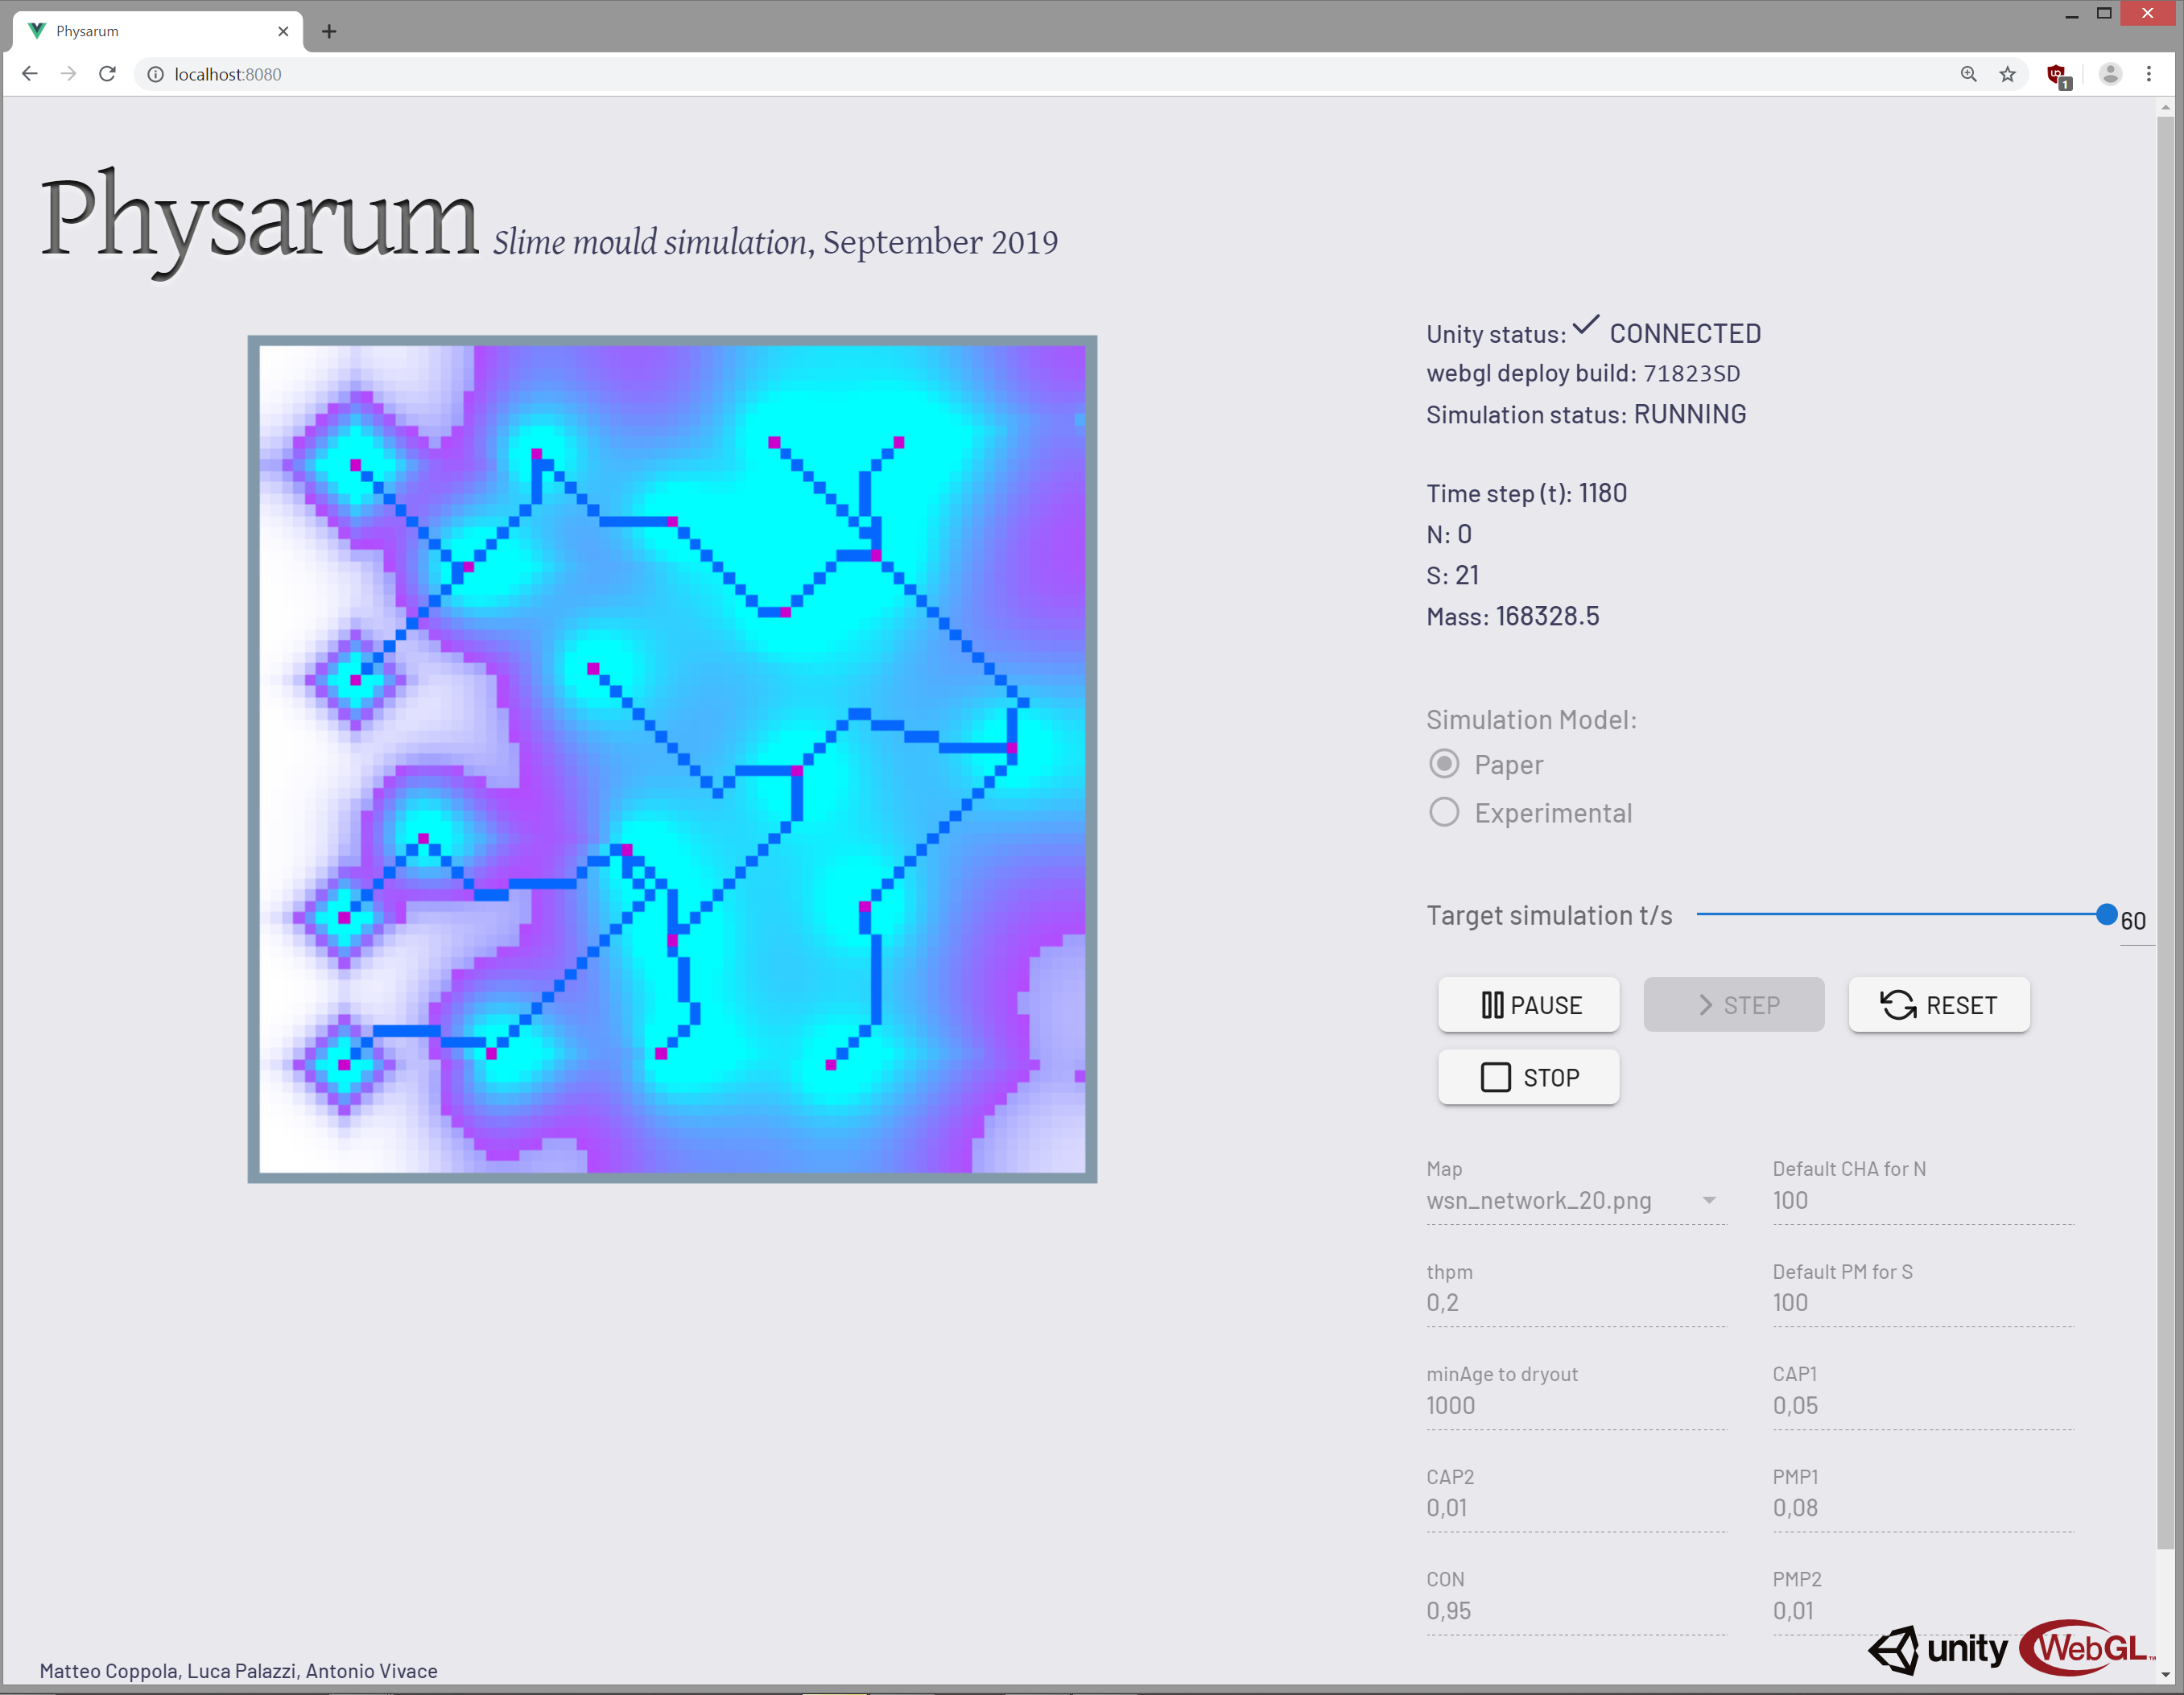
\includegraphics[width=0.8\textwidth]{UI1}%
    
  \caption{Final application view}
  \label{fig:swstack1}
\end{figure*}

\begin{figure*}
  \centering
    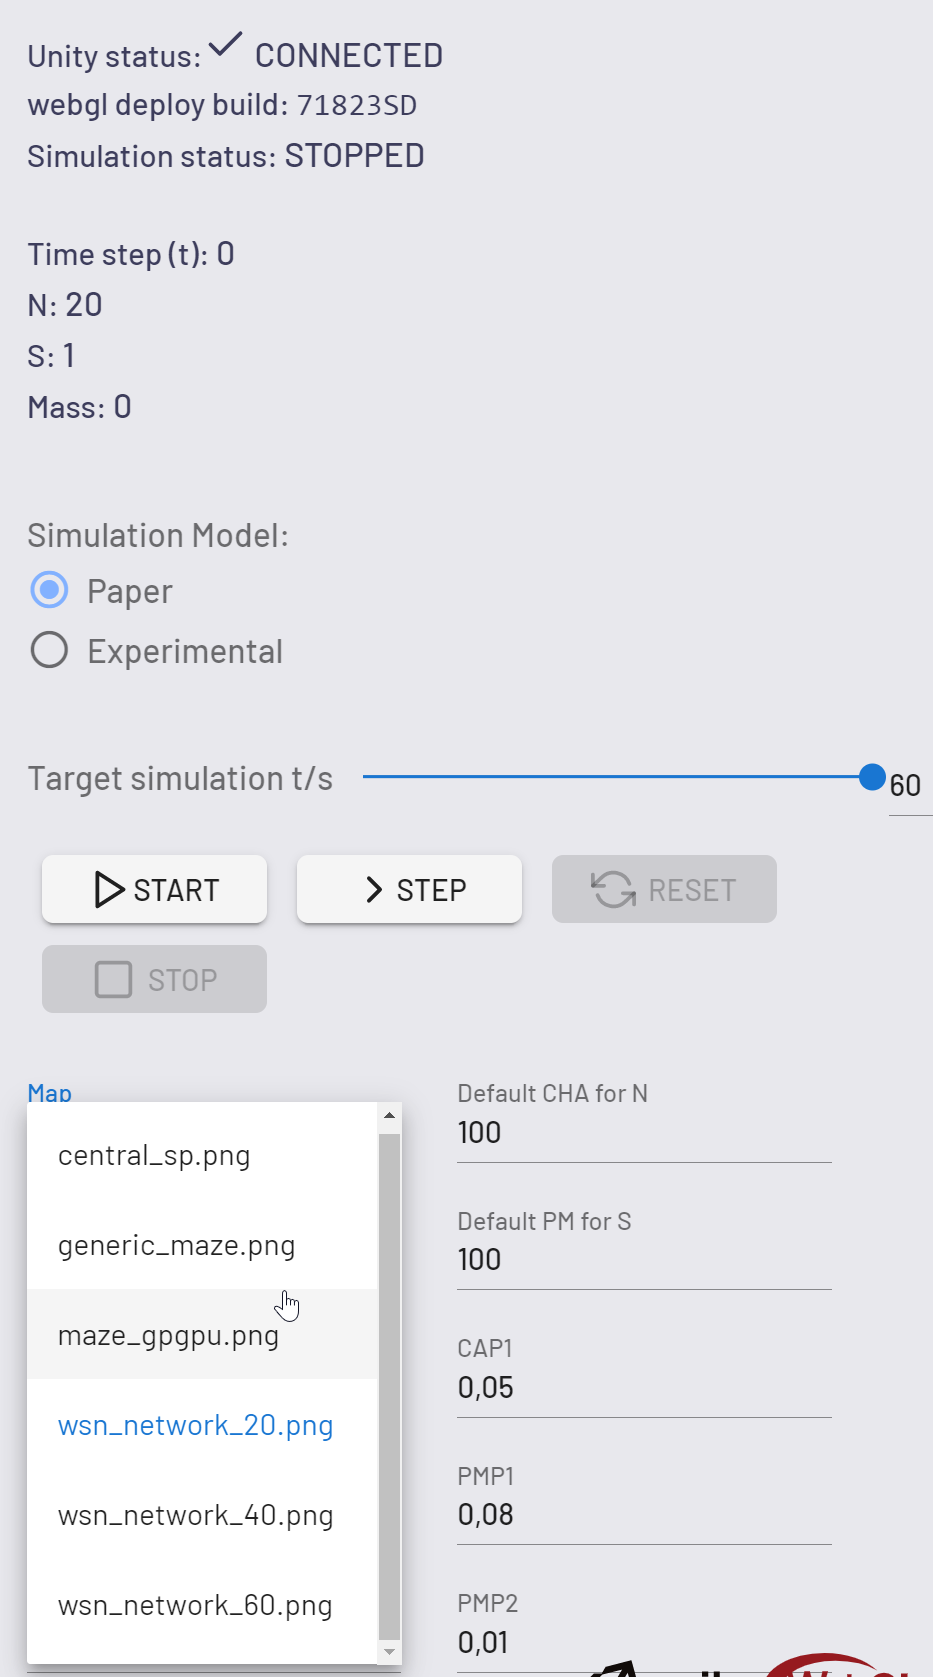
\includegraphics[width=0.4\textwidth]{UI2}%
    
  \caption{User Interface view}
  \label{fig:swstack1}
\end{figure*}

\section{Simulation framework}
\begin{figure*}
  \centering
    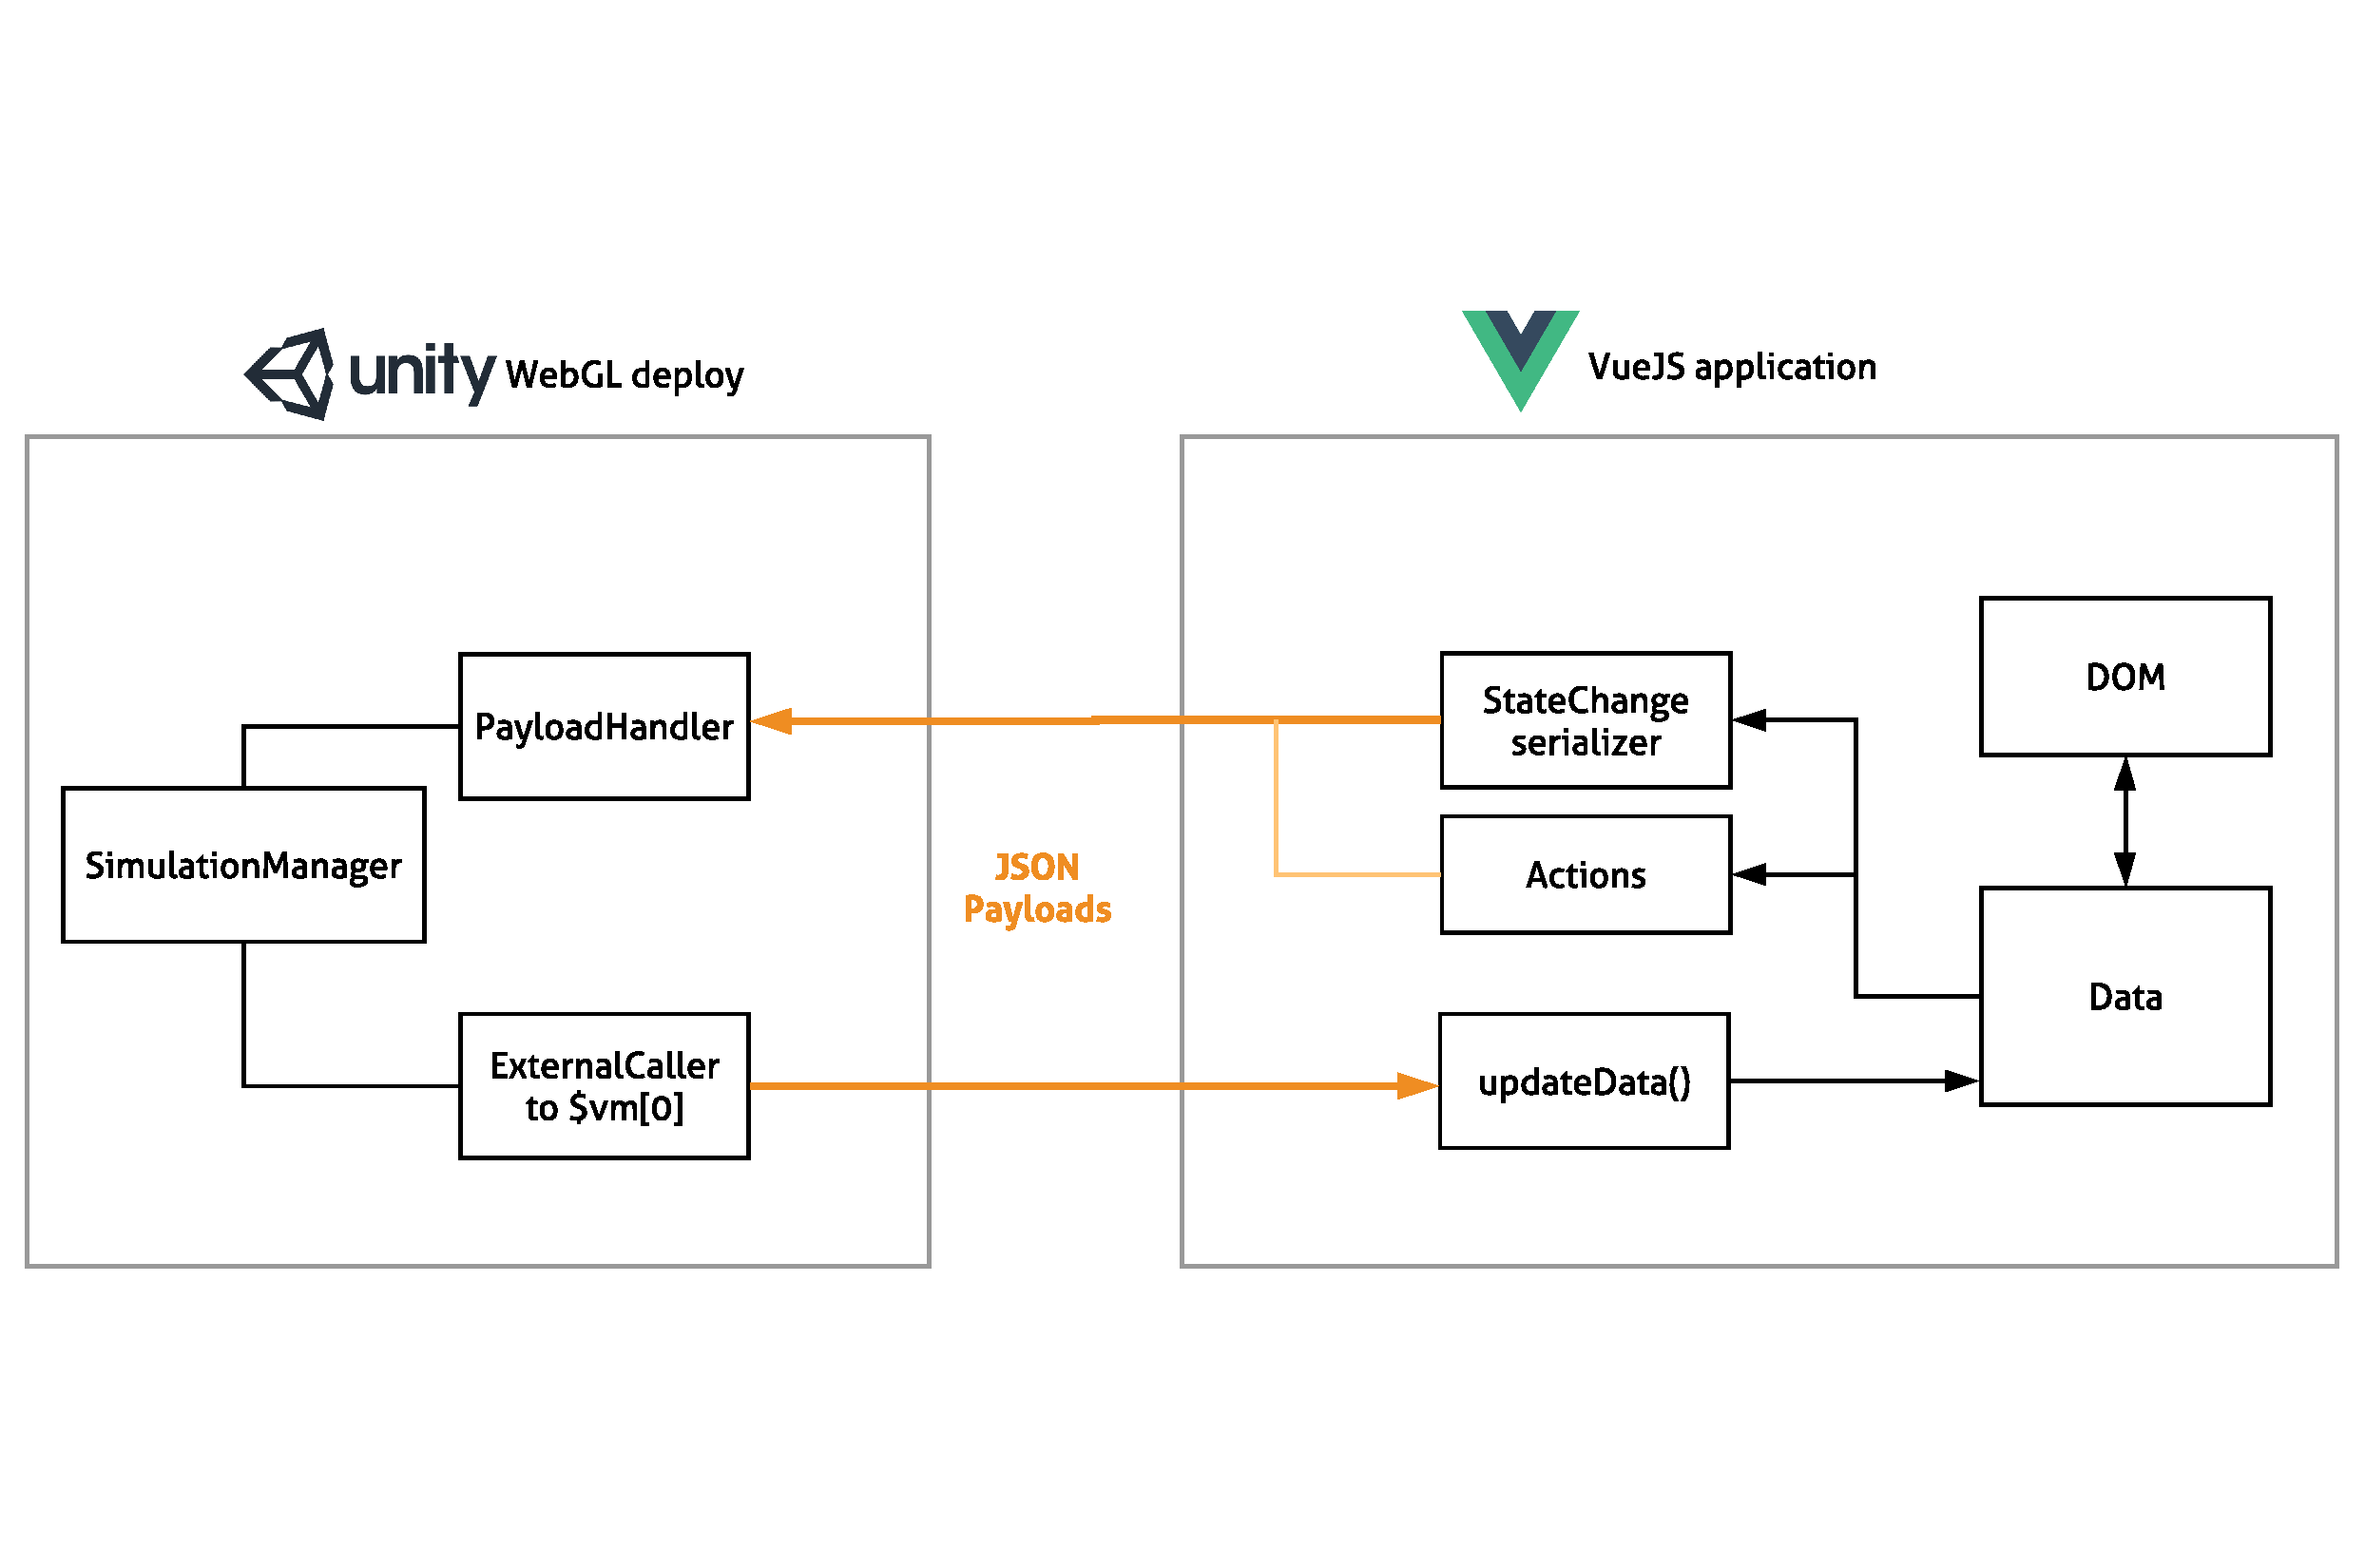
\includegraphics[width=1\textwidth]{sw_arch}%
    
  \caption{Overview of the implemented VueJS - Unity bidirectional comunication}
  \label{fig:swstack1}
\end{figure*}
\subsection{Vue and Unity bidirectional communication}
After some initial experimentation, Unity emerged as suitable for the described requisites, it run fast, and defining local rules for the evolving values of the parameters for each cells was easy and immediate.

Adding Vuetify, a CSS framework providing ready UI components, to Vue.js allowed us to design a good looking and functional user interface, exposing execution control buttons, inputs and select forms to monitor and control each aspect of the simulation.

However, we needed a fast and realiable way to make those two components comunicate constantly and in both directions:

\paragraph{Vue to Unity}

When Unity is loaded, it exposes a \texttt{gameInstance} object. We can use the \texttt{SendMessage} method offered by this object to launch a public method defined inside the Unity scripts directly from the webpage embedding that Unity application. This is simple and allows passing integers and string arguments.

E.g. the following line is called by Vue whenever the \texttt{onChange} even is triggered by the FPS slider:

\begin{verbatim}
gameInstance.SendMessage("GameObject", "changeFrameRate", this.fps)
\end{verbatim}

We call the \texttt{changeFrameRate} Unity method passing the new desired framerate:

\begin{verbatim}
void changeFrameRate(int targetFps){
    Application.targetFrameRate = targetFps;
}
\end{verbatim}

\paragraph{Unity to Vue}

When the browser finishes the loading of the Vue framework, the instance becomes available as \texttt{vm.\$children[0]} and we can call any of the function exposed as "method" inside the Vue definition with this object.
In Unity, we have a \texttt{Application.ExternalCall} function which calls functionName in the web page containing the WebGL player, passing the given arguments to it. Supported argument types are the primitive types (string, int, float, string) and arrays of such types.

E.g. this is the Unity function that sends to the UI the current values of the simulation:

\begin{verbatim}
void updateParameters(){
    Application.ExternalCall("vm.$children[0].unityParamUpdate",
        defaultPMForS,
        defaultCHAForN,
        CON,
        CAP1,
        CAP2,
        ThPM,
        minAgeToDryOut,
        PMP1,
        PMP2);
}
\end{verbatim}

On Vue, this function simply acts as settern, updating its internal values with the one provided. It's defined as follows:

\begin{verbatim}
unityParamUpdate(defaultPMForS,
    defaultCHAForN,
    CON,
    CAP1,
    CAP2,
    ThPM,
    minAgeToDryOut,
    PMP1,
    PMP2){
        this.defaultPMForS = defaultPMForS;
        this.defaultCHAForN = defaultCHAForN;
        this.CON = CON;
        this.CAP1 = CAP1;
        this.CAP2 = CAP2;
        this.ThPM = ThPM;
        this.minAgeToDryOut = minAgeToDryOut;
        this.PMP1 = PMP1;
        this.PMP2 = PMP2;
},
\end{verbatim}


Exploiting these two simple patterns, we can communicate and synchronize the two application logics. From the UI we can:

\begin{itemize}
\item Start, Stop and pause the simulation;
\item Stop and reset the simulation with the default values;
\item Run just one step at the time of the simulation;
\item Change the application target time steps/seconds;
\item Change map;
\item Change the simulation model;
\item Change the simulation parameters.
\end{itemize}

While from Unity we

\begin{itemize}
    \item Show the simulation tilemap;
    \item Send updated values about the simulation at each frame;
    \item Send the updated parameters values.
\end{itemize}

\subsection{More complex payloads}

An additional JSON serializer/deserializer class was developed even if it eventually resulted easier and clearer to just pass every parameter in a stringified array instead of building an ad-hoc Payload class with each needed property every time. 

However, this approach is much more scalable and will definitely be useful in bigger applications, e.g. when the Payload between the two components will need to carry complex and heavier (maybe binary) data such as entire custom maps.

\subsection{Developoment and deployment}

The development of the application was done on UNIX systems, using git as version control system.

Webpack is a module builder for recent web technologies, a template configuration is provided with Vue: it provides hot reload and a development server to see the application live in the browser and automatically rebuilt on each change on the Vue side.

The Unity application must be built using the WebGL target. The build artifacts must be served statically by the web application, so we can embed the UnityPlayer and the actual application alongside the VueJS instance.

GitHub, our git hosting of choice, allows to serve static webpages. We exploited this functionality to obtain an easy and fast way to continuosly deploy our application: a simple script (\texttt{npm deploy}) build the Vue.JS application for production (with the Unity webGL build artifacts as static assets), then deploys it on the "master" branch of the repository. GitHub then serves the contents of this branch with its free service GitHub Pages.

\section{Simulation lifecycle}


EVENTS 


\subsection{Color shading}

One of the most important aspect of the simulation is how to present the results, in real time and in a meaningful and intuitive way. 

We wanted to put focus on one particular feature: the transition of the mass among cells, both on the smaller and the outer range.

This means we needed a smooth animation, making use a changing color tone, representing the steady and consistent movement and formation of the slime mould navigating the map, while expressing how the mass density was changing and moving among areas.

\paragraph{Linear interpolation approach}

The initial approach we considered was a standard linear interpolation: assuming colors are given as triples $(r_1,g_1,b_1)$ and $(r_2,g_2,b_2)$ in the RGB color system, we can fade between them with a simple \textit{linear interpolation}:

\begin{align}
r' &= (1-t)\cdot r_1+t\cdot r_2\\
g' &= (1-t)\cdot g_1+t\cdot g_2\\
b' &= (1-t)\cdot b_1+t\cdot b_2
\end{align}

This gives a blended color $(r',g',b')$ for all $t\in[0,1]$. For $t=0$ it will give the first color, for $t=1$ the second color.


$$ C_1=\begin{pmatrix}r_1\\g_1\\b_1\end{pmatrix}, \qquad C_2=\begin{pmatrix}r_2\\g_2\\b_2\end{pmatrix}$$

The blended color is given as the vector $C'(t)=(1-t)\cdot C_1+t\cdot C_2$.


\begin{figure*}
  \centering
    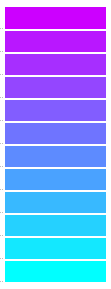
\includegraphics{colorshade1}%
    
  \caption{The chosen color shading}
  \label{fig:color}
\end{figure*}


\paragraph{Prescaling and tuning}

The value we want to represent with color is the \textit{Mass} of every single cell. This values varies greatly (and with a different rate based on the model), but we're particularly interested in the growth of smaller values (the mould exploring) and the internal movement of mass.

The different rate of growth is taken into account using two different prescale factors: the mass on the Paper model is reduced by a factor of 50, while ours is reduced by a factor of 10.

We also don't want to represent any value exceeding a threshold since nothing interesting happens after a certain value, and we do not want to focus on something not effecting the actual behaviour of the simulation. This threshold was set to 1000 for the Paper simulation and 100 for the experimental one.

\paragraph{Chosen color shading algorithm}

Following the ideas of the linear interpolation, our color shading algorithms works in the following way. We express colors in Unity's class using RGB triples, with each value in the 0-1 range.\\

PaperModel:

\begin{itemize}
    \item Empty cells are white. C= $(1,1,1)$
    \item Cell mass is scaled with a factor of 50 (40 on low-mass cells). $PM = PM/50$
    \item On low-mass cells ($PM < 15$): C= $(1-PM,1-PM,1)$
    \item C= $(1-PM,PM,3)$
\end{itemize}

Experimental Model:

\begin{itemize}
    \item Empty cells are white.
    \item Cell mass is scaled with a factor of 10. $PM = PM/10$
    \item C= $((0.8-PM)*1.25,(PM-0.20)*1.25,1)$
\end{itemize}

The result is shade of light blue to blue-purple where the lighter values represent more action, more mass and general more mass movement activity, while the darker are the expansion front of the slime mould. The color range is also confined in a precise range (light blue to purple) with offsets on the Red and Green component of the color.

\paragraph{Additional expanding shading for the Paper simulation}

Since the paper simulation is expading extremely fast with a very low amount of mass, each run launched with our color shading algorithm was immediatly flooding the entire map, making the color shading pretty much useless until the mass started to grow near the S points.

So, for the lower values, we chosen to represent the initial expansion with another color shading formula, giving a very subtle (and almost transparent) shade of blue around the front of expansion of the slime mould.

\chapter{Simulations}
\label{simulations}

Physarum presents the intelligence of finding effective solutions to demanding engineering problems such as shortest path problems, various graph problems, evaluation of transport networks or even robotic control.
The most well-known laboratory experiments that the plasmodium of slime mould is subjected to are the imitation and optimization of human-made transport networks and the finding of the shortest path in a maze.
Part of our project is to verify the effective functioning of each model and compare the results obtained simulating the slime mould in predefinite maps.

\par
Our simulations are based on the work of the same research group \cite{dourvas2016gpgpu}, \cite{tsompanas2015cellular} that have reproposed the diffusion equations of the original model \cite{Tsompanas2016} and then have applied those in different contexts.

\par
The model of Tsompanas et al. \cite{Tsompanas2016} has some important alternation from the others cited. In particular, the same diffusion equations are incorporated in an algorithm composed by the following steps:

\begin{enumerate}
	\item Initialize the model: the parameters of the diffusion equations are set and the topology of the SP and the NSs is also introduced
	\item Apply the diffusion equations for 50 time steps
	\item Check if any of the NSs is covered with a predefined percentage of PM (ThPM). If there is at least one NS covered continue, else go to (2).
	\item All NSs covered with the predefined percentage of PM (ThPM), are encapsulated by the plasmodium and therefore connected to a SP.
	\item The NSs mentioned in (4) change into SPs, meaning their PM is set to 100. If no more than 5,000 time steps have passed (t <5,000) go to (2), else continue.
	\item Redefine all the cells of “interest” (NSs and SP) as NSs, except from the second to last NS encapsulated for the previous 5,000 time steps which is redefined as a SP. Execute for a second time (2)–(5) for 5,000 time steps.
\end{enumerate}

Note that some procedures are identical for each work previously analyzed \cite{dourvas2016gpgpu}, \cite{tsompanas2015cellular}. We firstly initialize the parameters, set one SP in the map as the beginning mass value of the plasmodium with a $PM$ value equals to 100 and then in one or more cell we set the NS which has a $CHA$ value equals to 100. Then, an iterative execution of the diffusion equations gives the values of $PM$ and $CHA$ for all the cells in the CA grid.

\par
From here on there are substancial differences in the approaches used. In \cite{dourvas2016gpgpu} and \cite{tsompanas2015cellular} the procedure stops and the algorithm designs the minimum tubular network based on the values of the $PM$ variable. When a cell’s $TE$ = \texttt{true} then the algorithm searches which of its neighbors has the greater value of $PM$. When it finds it, the $TE$ value of neighbor changes from \texttt{false} to \texttt{true}. This procedure is repeated until the final, minimum tube is created between the cell that the plasmodium was first introduced to the cell with the $NS$. 

\par
In \cite{Tsompanas2016}, in addition, there's the last step of the algorithm explained above that is tricky. It redefine all the NSs and SP as NSs, except from the second to last NS encapsulated for the previous 5000 time steps which is redefined as a SP. This happen because as the CA model is designed without the use of probabilistic equations, it uses a second starting point to regenerate and explore the available area once more. That point will be a point of interest (NS), which is empirically chosen to be away from the initial SP. The second to last NS to be encapsulated was chosen, based on the fact that it is far enough from the initial SP and it is less likely to be a point of interest surrounded by unavailable area that would cause difficulties for the growth of the plasmodium. Then this model requests a second time execution of the algorithm steps from 2 to 5 for further 5000 time steps.

\par
This last part of seems to be forced considering, as we will see in the next sections related to the simulations, that a certain point the computation arrives at a steady state in which the $PM$ covers the map completely with the same value, leading then to a steady state. As mentioned in \cite{dourvas2016gpgpu} usually about a 1700 time steps are required for the CA-modeled plasmodium to explore a $75 \times 75$ map.

\section{Network formation}
\label{network_formation_5}
In order to evaluate the efficiency of the networks of the bioinspired CA based model, randomly deployed distributions of 20, 40 and 60 nodes are evaluated. The maps are proposed below:

\begin{figure}[H]
  \centering
    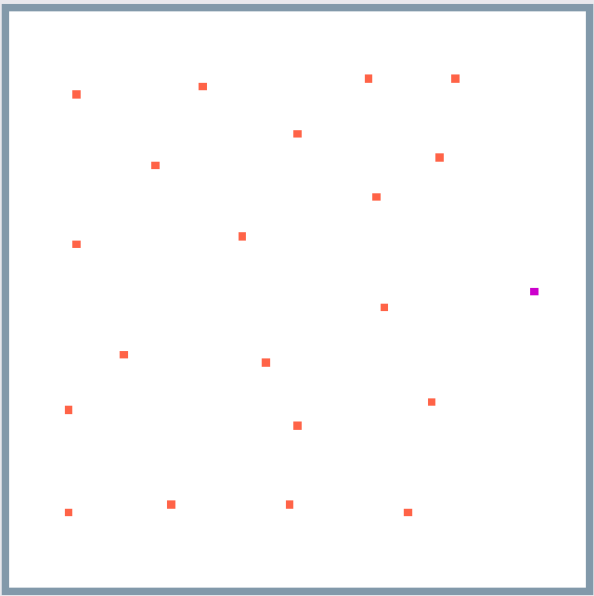
\includegraphics[width=0.48\textwidth]{wsn_20_exp/1_wsn_20}%
    
  \caption{Wsn network with 20 nodes}
  \label{fig:wsn_20_exp/1_wsn_20}
\end{figure}

\begin{figure}[H]
  \centering
    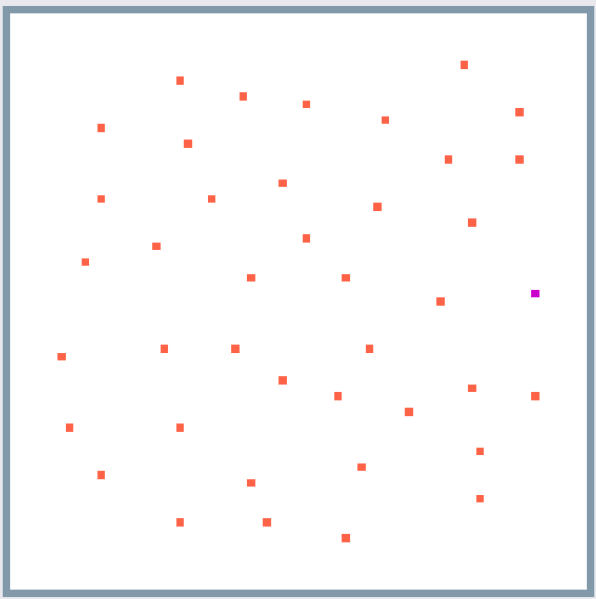
\includegraphics[width=0.48\textwidth]{wsn_40_exp/1_wsn_40}%
    
  \caption{Wsn network with 40 nodes}
  \label{fig:wsn_40_exp/1_wsn_40}
\end{figure}

\begin{figure}[H]
  \centering
    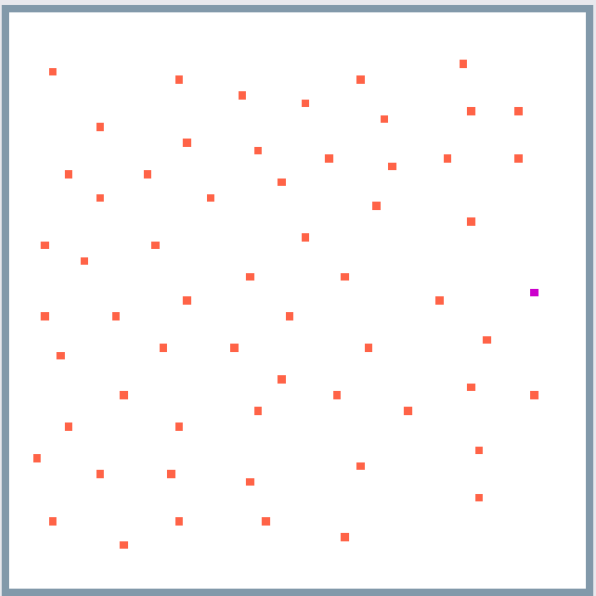
\includegraphics[width=0.48\textwidth]{wsn_60_exp/1_wsn_60}%
    
  \caption{Wsn network with 60 nodes}
  \label{fig:wsn_60_exp/1_wsn_60}
\end{figure}

These maps are very similar to those proposed in \cite{tsompanas2015cellular} in which the plasmodium of Physarum polycephalum is the inspiration of a CA based model for constructing data trees in a WSN that connect all nodes with a sink node, that is located in the east border of the WSN for each of the three distributions.

\par
The black dot illustrates the location of the sink node and the yellow dots illustrate the locations of the sensing nodes. The topologies of the nodes are used as input for the model, with the sink node represented as the SP and all the other nodes represented as NSs. Furthermore, the initial parameters set for the model are illustrated in the next subsections.

\par
In addition to the previous maps we have also considered as an experiment a network with SP in a centered position, as can be seen in figure~\ref{fig:central_sp_exp/1_central_sp}.

\begin{figure}[H]
  \centering
    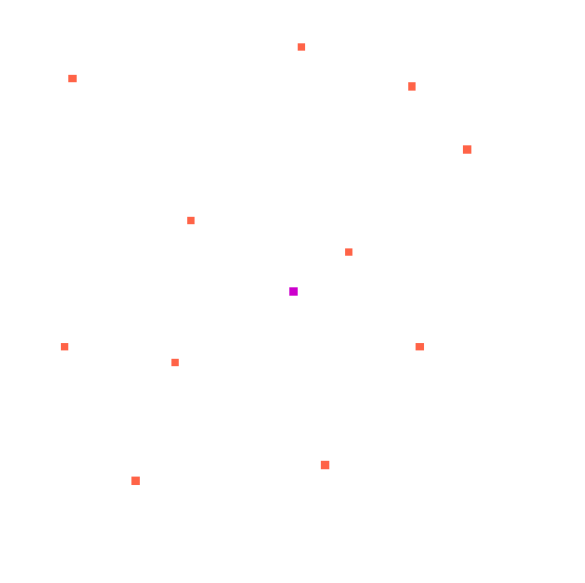
\includegraphics[width=0.48\textwidth]{central_sp_exp/1_central_sp}%
    
  \caption{Network with SP in a centered position}
  \label{fig:central_sp_exp/1_central_sp}
\end{figure}

\subsection{Paper model}

In this case the parameters are the same for each of the four networks simulated.

\begin{center}
 \begin{tabular}{||c c||} 
 \hline
 Parameter & Value \\ [0.5ex] 
 \hline\hline
 GridSize & $75 \times 75$ \\ 
 \hline
 PM & 100 \\ 
 \hline
 CHA & 100 \\ 
 \hline
 CON & 0.95 \\ 
 \hline
 PAP & 0.8 \\ 
 \hline
 PMP1 & 0.08 \\ 
 \hline
 PMP2 & 0.01 \\ 
 \hline
 CAP1 & 0.05 \\ 
 \hline
 CAP2 & 0.01 \\ 
 \hline
 ThPM & 0.2 \\ [1ex] 
 \hline
 \end{tabular}
\end{center}

Below are shown the simulation for each network. 

\begin{figure}[H]
    \centering
    \subfigure[Expansion process]{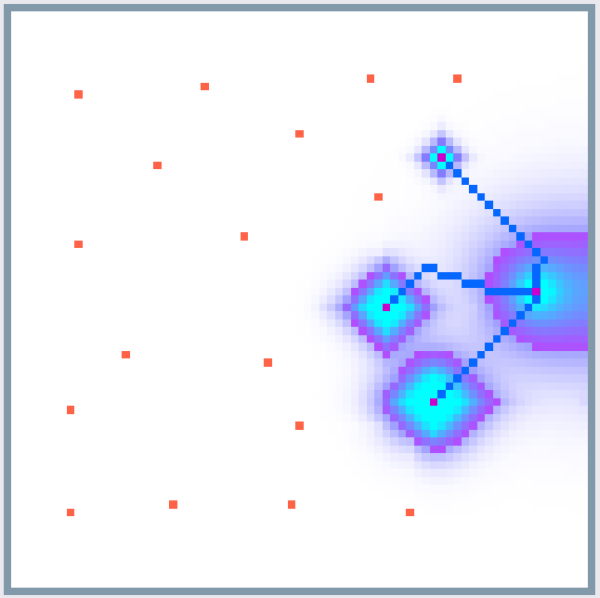
\includegraphics[width=0.40\textwidth]{wsn_20_pap/2_wsn_20}}
    \subfigure[Simulation end]{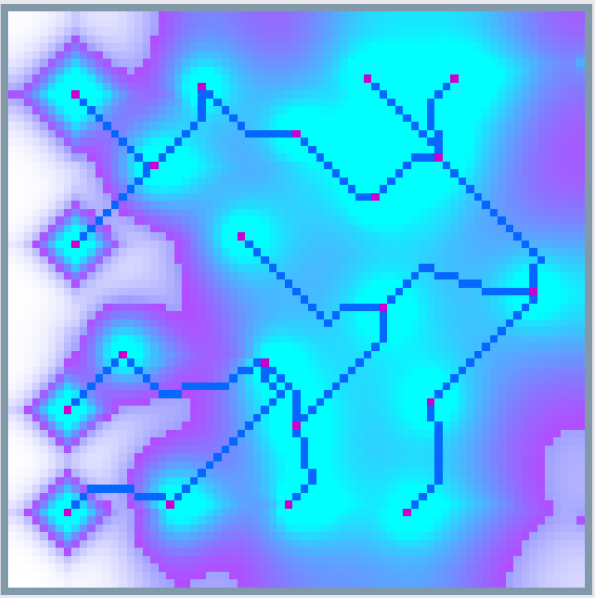
\includegraphics[width=0.40\textwidth]{wsn_20_pap/3_wsn_20}}
    \caption{Wsn network with 20 NSs}
    \label{fig:foobar}
\end{figure}


\begin{figure}[H]
    \centering
    \subfigure[Expansion process]{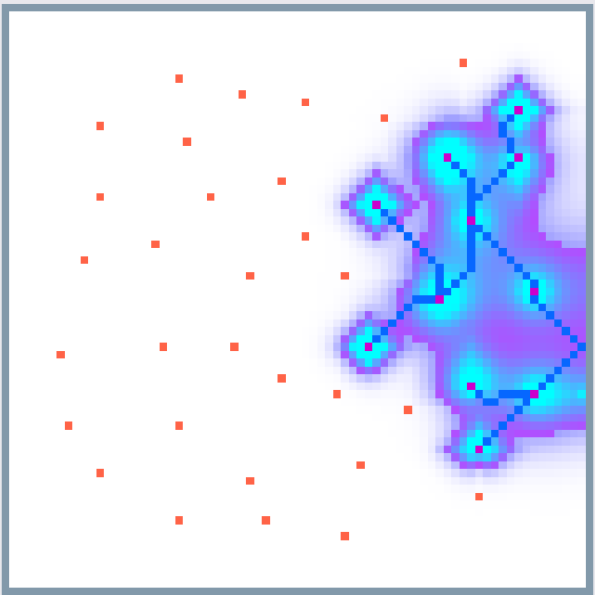
\includegraphics[width=0.40\textwidth]{wsn_40_pap/2_wsn_40}} 
    \subfigure[Simulation end]{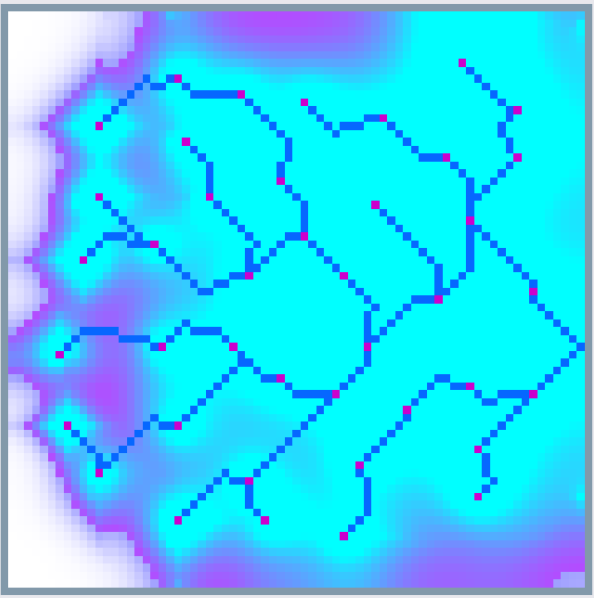
\includegraphics[width=0.40\textwidth]{wsn_40_pap/3_wsn_40}} 
    \caption{Wsn network with 40 NSs}
    \label{fig:foobar}
\end{figure}

\begin{figure}[H]
    \centering
    \subfigure[Expansion process]{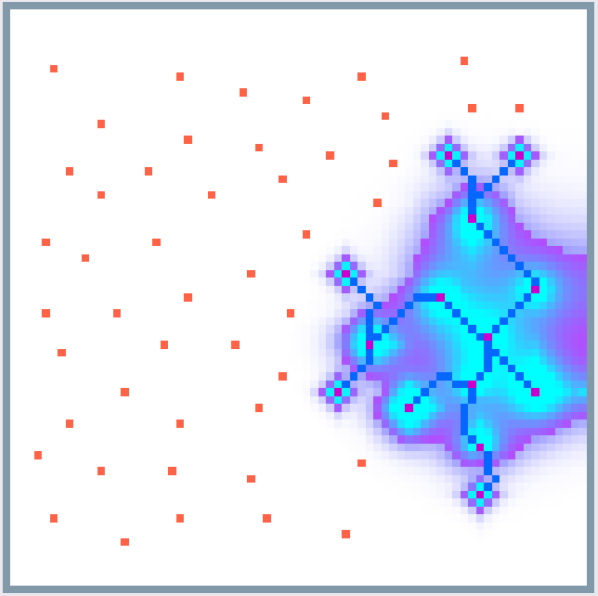
\includegraphics[width=0.40\textwidth]{wsn_60_pap/2_wsn_60}} 
    \subfigure[Simulation end]{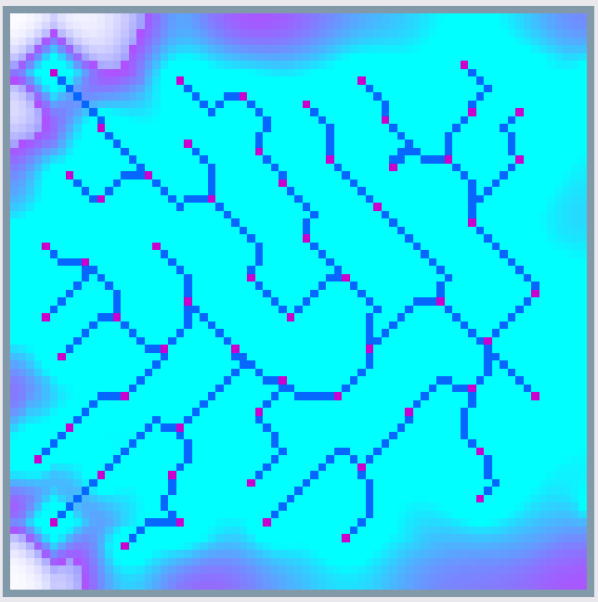
\includegraphics[width=0.40\textwidth]{wsn_60_pap/3_wsn_60}} 
    \caption{Wsn network with 60 NSs}
    \label{fig:foobar}
\end{figure}

\begin{figure}[H]
    \centering
    \subfigure[Expansion process]{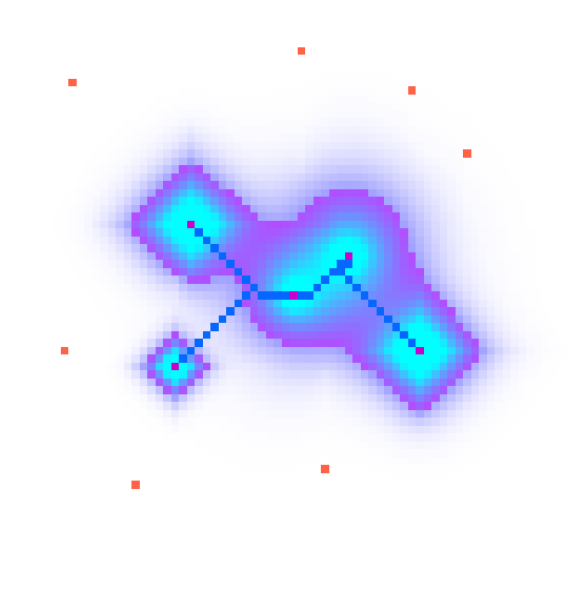
\includegraphics[width=0.40\textwidth]{central_sp_pap/2_central_sp}} 
    \subfigure[Simulation end]{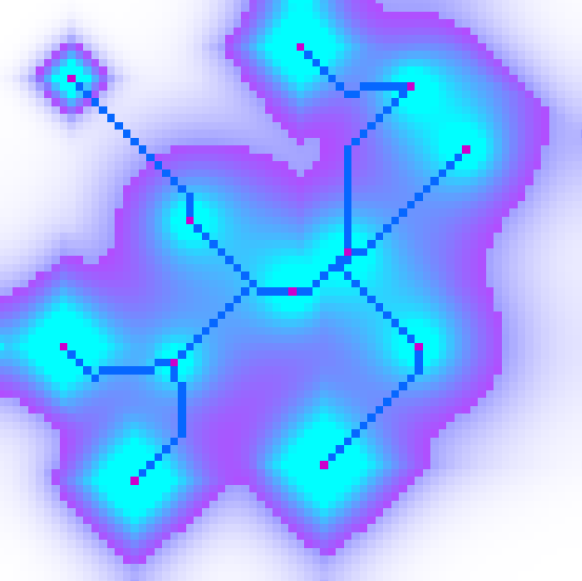
\includegraphics[width=0.40\textwidth]{central_sp_pap/3_central_sp}} 
    \caption{Network with SP in a centered position}
    \label{fig:foobar}
\end{figure}

\subsection{Experimental model}

Also in this case the parameters are the same for each of the four maps simulated.

\begin{center}
 \begin{tabular}{||c c||} 
 \hline
 Parameter & Value \\ [0.5ex] 
 \hline\hline
 GridSize & $75 \times 75$ \\ 
 \hline
 PM & 10000 \\ 
 \hline
 CHA & 100 \\ 
 \hline
 CON & 0.95 \\ 
 \hline
 CAP1 & 0.05 \\ 
 \hline
 CAP2 & 0.01 \\ 
 \hline
 MinAgeDryOut & 1000 \\
 \hline
 ThPM & 20 \\ [1ex] 
 \hline
 \end{tabular}
\end{center}

Below are shown the simulations for each map. 

\begin{figure}[H]
    \centering
    \subfigure[Expansion process]{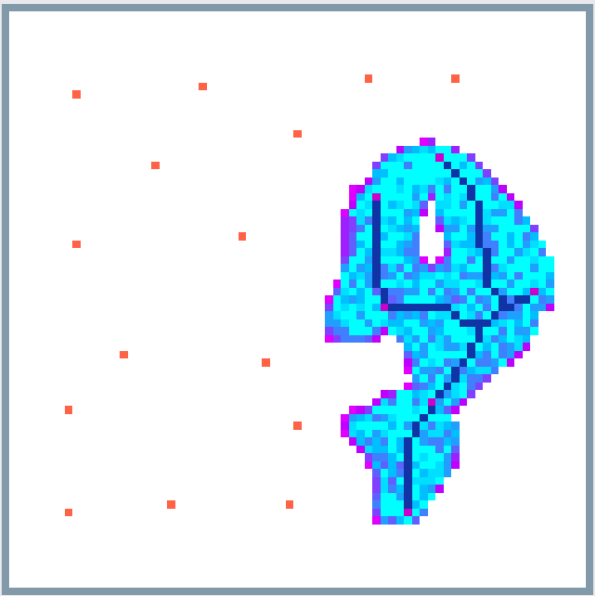
\includegraphics[width=0.32\textwidth]{wsn_20_exp/2_wsn_20}} 
    \subfigure[Shrinking process]{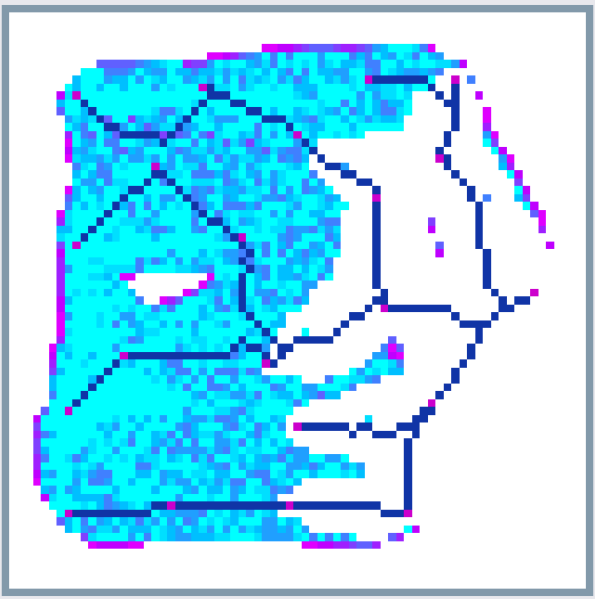
\includegraphics[width=0.32\textwidth]{wsn_20_exp/3_wsn_20}} 
    \subfigure[Simulation end]{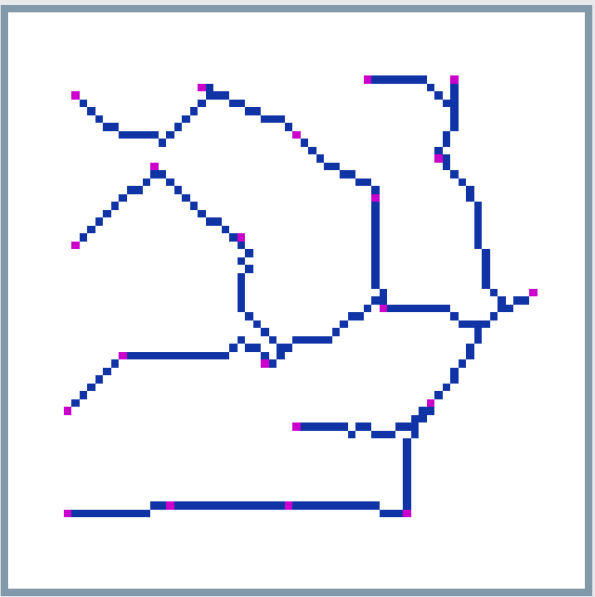
\includegraphics[width=0.32\textwidth]{wsn_20_exp/4_wsn_20}}
    \caption{Wsn network with 20 NSs}
    \label{fig:foobar}
\end{figure}

\begin{figure}[H]
    \centering
    \subfigure[Expansion process]{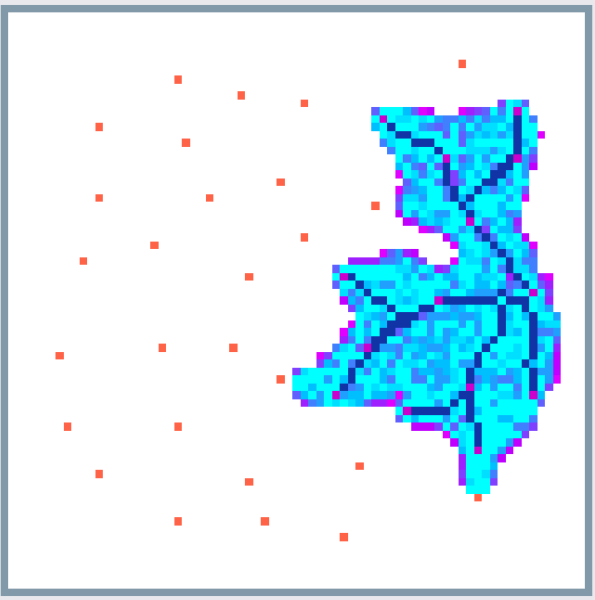
\includegraphics[width=0.32\textwidth]{wsn_40_exp/2_wsn_40}} 
    \subfigure[Shrinking process]{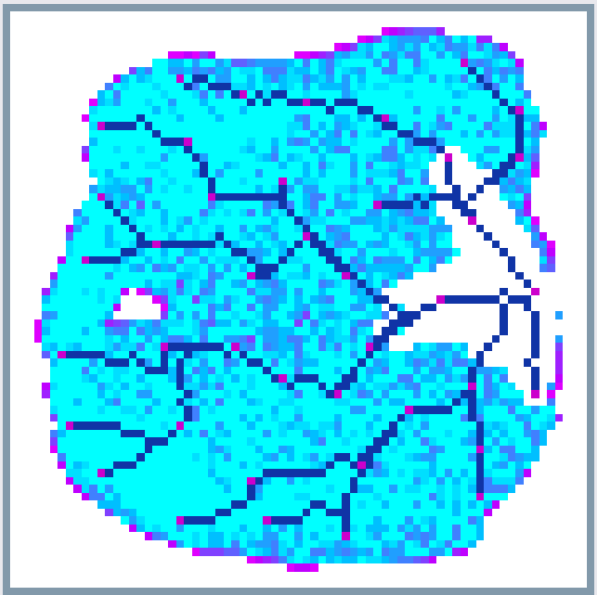
\includegraphics[width=0.32\textwidth]{wsn_40_exp/3_wsn_40}} 
    \subfigure[Simulation end]{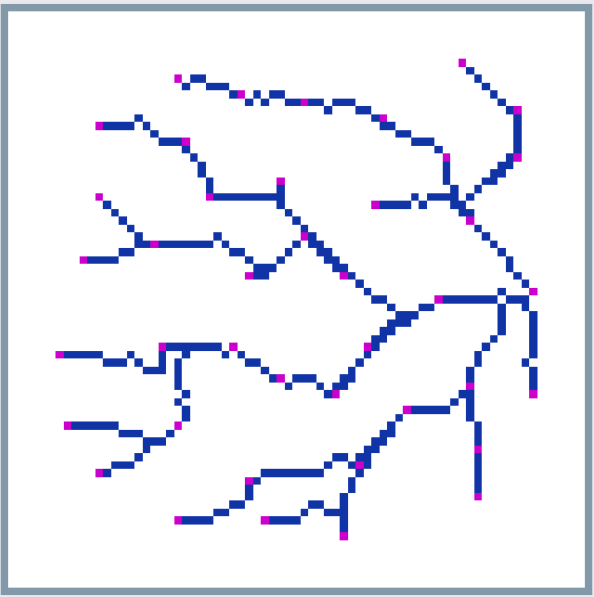
\includegraphics[width=0.32\textwidth]{wsn_40_exp/4_wsn_40}}
    \caption{Wsn network with 40 NSs}
    \label{fig:foobar}
\end{figure}

\begin{figure}[H]
    \centering
    \subfigure[Expansion process]{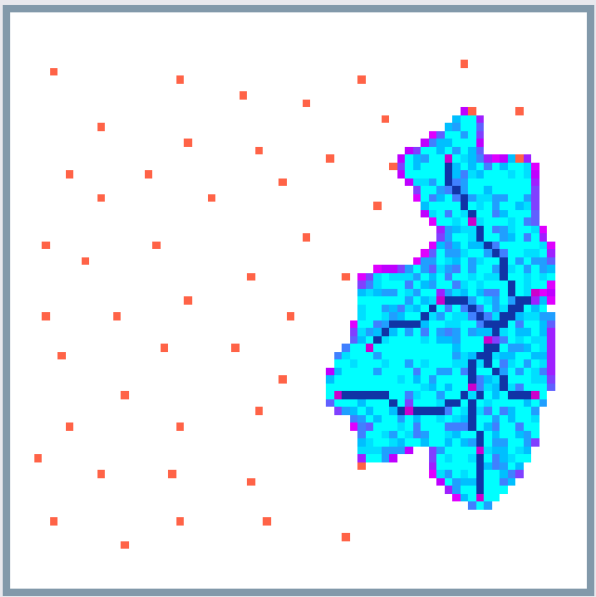
\includegraphics[width=0.32\textwidth]{wsn_60_exp/2_wsn_60}} 
    \subfigure[Shrinking process]{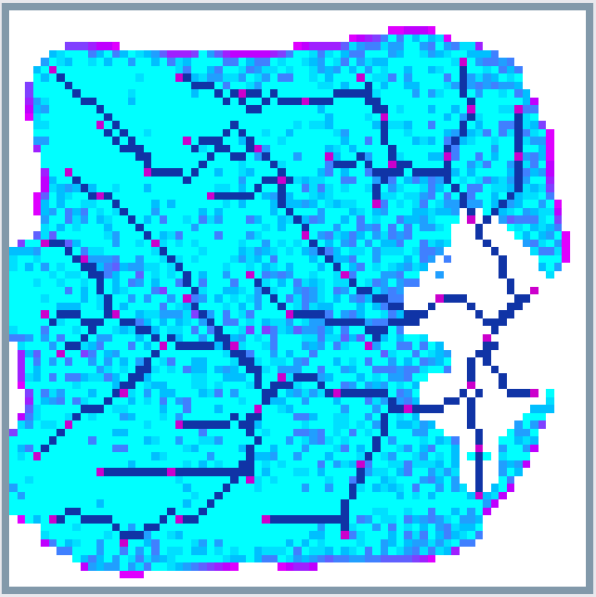
\includegraphics[width=0.32\textwidth]{wsn_60_exp/3_wsn_60}} 
    \subfigure[Simulation end]{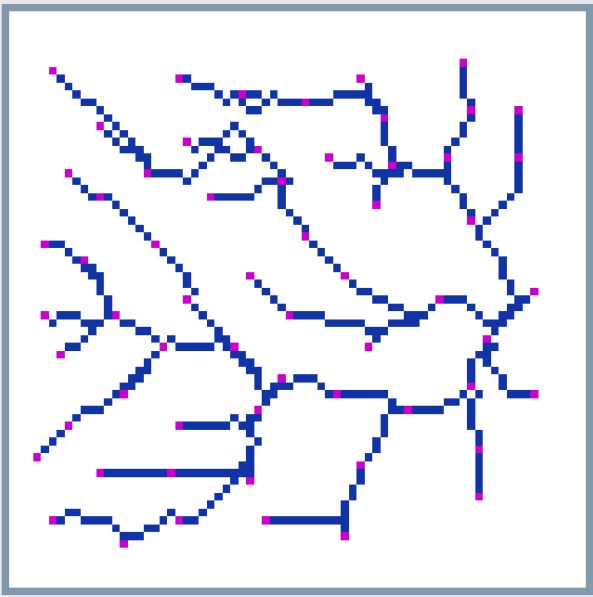
\includegraphics[width=0.32\textwidth]{wsn_60_exp/4_wsn_60}}
    \caption{Wsn network with 60 NSs}
    \label{fig:foobar}
\end{figure}

\begin{figure}[H]
    \centering
    \subfigure[Expansion process]{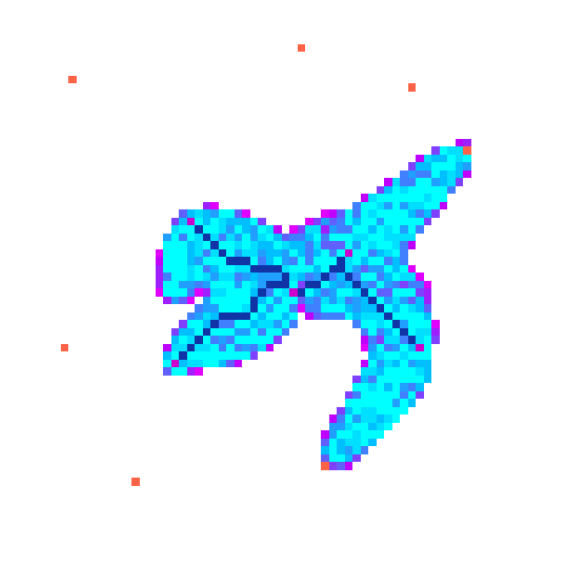
\includegraphics[width=0.32\textwidth]{central_sp_exp/2_central_sp}} 
    \subfigure[Shrinking process]{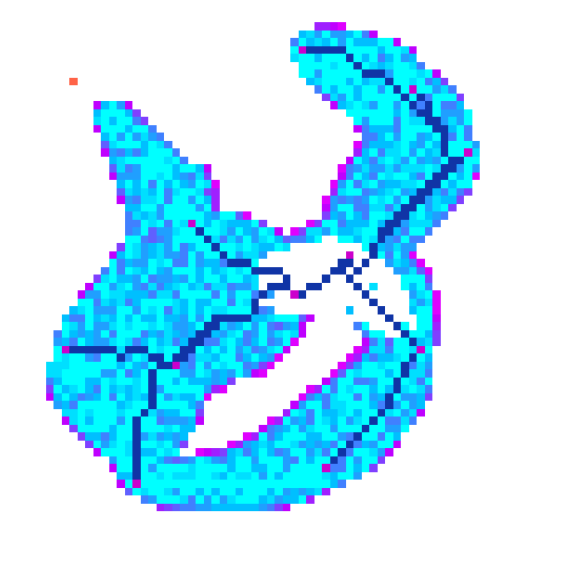
\includegraphics[width=0.32\textwidth]{central_sp_exp/3_central_sp}} 
    \subfigure[Simulation end]{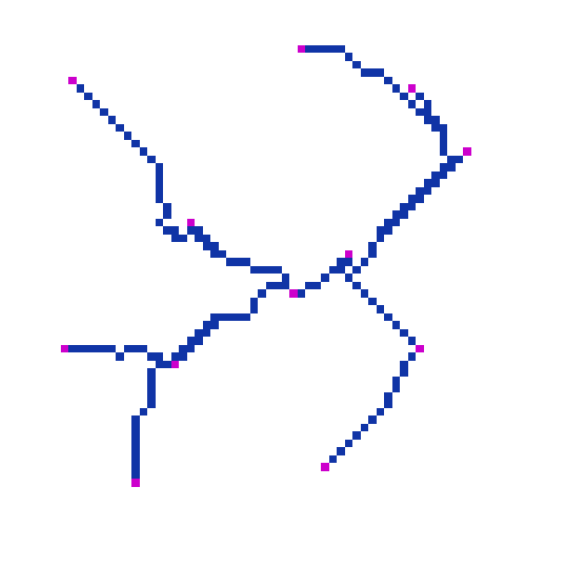
\includegraphics[width=0.32\textwidth]{central_sp_exp/4_central_sp}}
    \caption{Network with SP in a centered position}
    \label{fig:foobar}
\end{figure}

\section{Maze solving}
\label{maze_solving}

For the maze solving problem using a Physarum as biological organism two different maps were used: the first maze was faithfully copied from \cite{dourvas2016gpgpu}, while for the second maze we were inspired by one of the most famous experiments \cite{nakagaki2000intelligence} that observed mould behaving like a intelligent organism able to find the minimum-length solution between two points in a maze. The maps in the initial state are proposed below:

\begin{figure}[H]
  \centering
    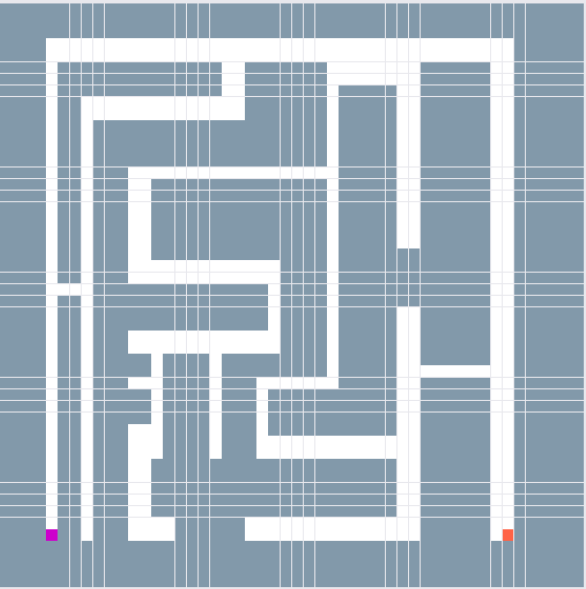
\includegraphics[width=0.48\textwidth]{maze_gpgpu_exp/1_maze_gpgpu}%
    
  \caption{First maze}
  \label{fig:maze_gpgpu_exp/1_maze_gpgpu}
\end{figure}

\begin{figure}[H]
  \centering
    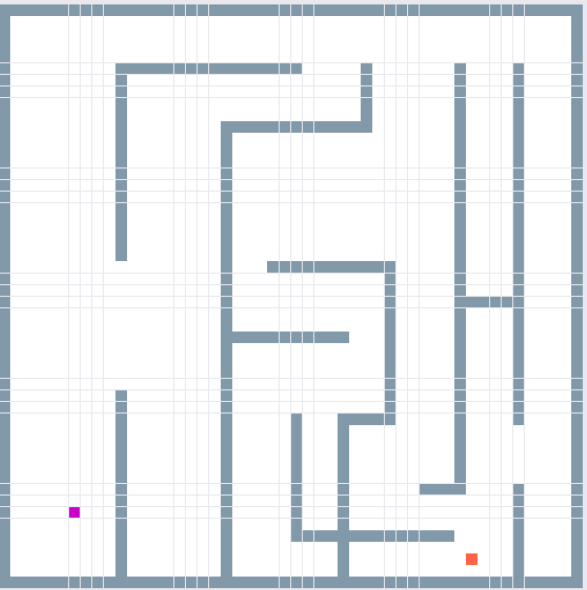
\includegraphics[width=0.48\textwidth]{generic_maze_exp/1_generic_maze}%
    
  \caption{Second maze}
  \label{fig:generic_maze_exp/1_generic_maze}
\end{figure}

Both maps are presented with an SP and an NS, respectively in the lower left corner and in the lower right corner and then at opposite sides of the maze.

\subsection{Paper model}
\label{paper_model}

For these maps the parameters are different from those applied in the maps representing a network, in particular as regards $PM$ and $CHA$ which are set to 30000 in \cite{dourvas2016gpgpu}.

\begin{center}
 \begin{tabular}{||c c||} 
 \hline
 Parameter & Value \\ [0.5ex] 
 \hline\hline
 GridSize & $50 \times 50$ \\ 
 \hline
 PM & 30000 \\ 
 \hline
 CHA & 30000 \\ 
 \hline
 CON & 0.95 \\ 
 \hline
 CAP1 & 0.05 \\ 
 \hline
 CAP2 & 0.01 \\ 
 \hline
 MinAgeDryOut & 1000 \\
 \hline
 ThPM & 20 \\ [1ex] 
 \hline
 \end{tabular}
\end{center}

\begin{figure}[H]
    \centering
    \subfigure[Max expansion]{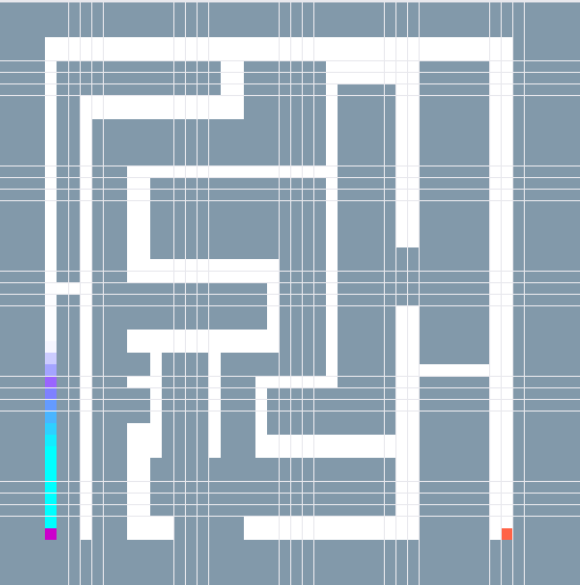
\includegraphics[width=0.40\textwidth]{maze_gpgpu_pap/2_maze_gpgpu}} 
    \subfigure[Regression]{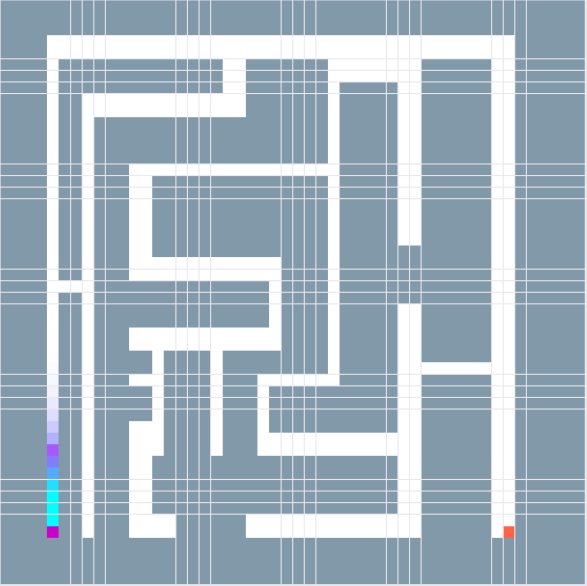
\includegraphics[width=0.40\textwidth]{maze_gpgpu_pap/3_maze_gpgpu}} 
    \caption{First maze}
    \label{fig:foobar}
\end{figure}

In this case the mould stops and begins to regress, failing to complete the maze. The simulation was also made by considerably increasing the initial mass, again achieving poor results.

\begin{figure}[H]
    \centering
    \subfigure[Expansion process]{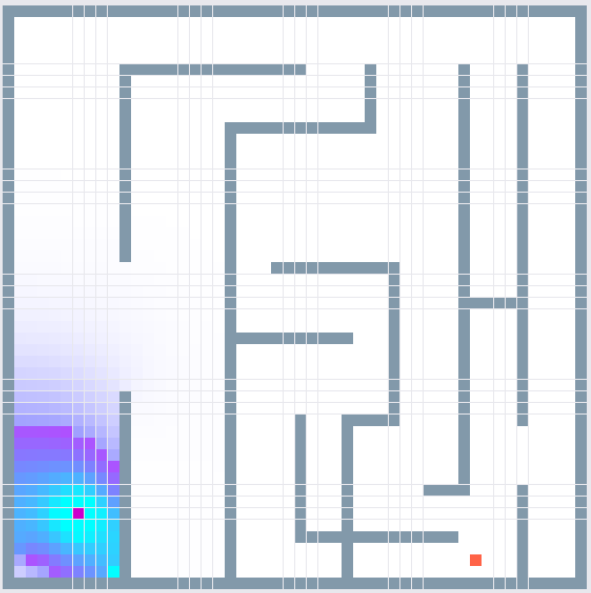
\includegraphics[width=0.40\textwidth]{generic_maze_pap/2_generic_maze}} 
    \subfigure[Last steps]{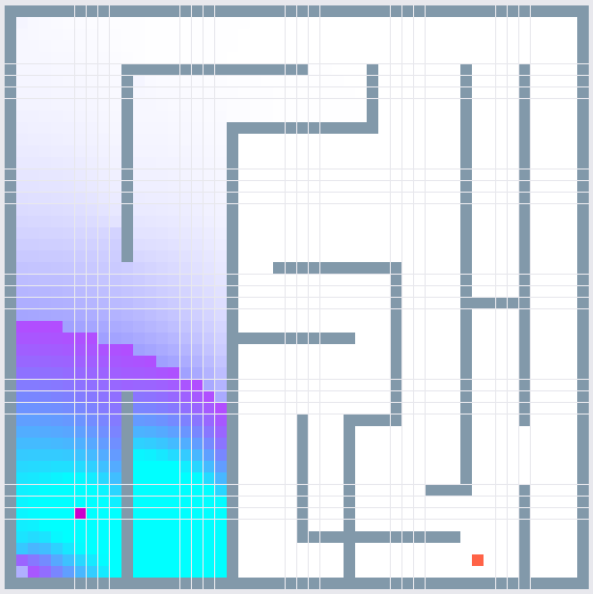
\includegraphics[width=0.40\textwidth]{generic_maze_pap/3_generic_maze}} 
    \caption{Second maze}
    \label{fig:foobar}
\end{figure}

In this another case the mould after 5050 steps has not yet reached the first NS. There is only one SP but we cannot change it into a NS.

\subsection{Experimental model}
\label{experimental_model}

In our model the mould manages to finish the mazes very well in both cases, but with a minimal difference in the MinAgeDryOut variable. Since the distance to be traveled is greater in the first maze, a greater value is needed which has been doubled bringing the value from 1000 of the second maze to 2000. The other values are equivalent for the success of the execution.

\paragraph{First maze}

\begin{center}
 \begin{tabular}{||c c||} 
 \hline
 Parameter & Value \\ [0.5ex] 
 \hline\hline
 GridSize & $50 \times 50$ \\ 
 \hline
 PM & 10000 \\ 
 \hline
 CHA & 100 \\ 
 \hline
 CON & 0.95 \\ 
 \hline
 CAP1 & 0.05 \\ 
 \hline
 CAP2 & 0.01 \\ 
 \hline
 MinAgeDryOut & 2000 \\
 \hline
 ThPM & 20 \\ [1ex] 
 \hline
 \end{tabular}
\end{center}

\begin{figure}[H]
    \centering
    \subfigure[Expansion process]{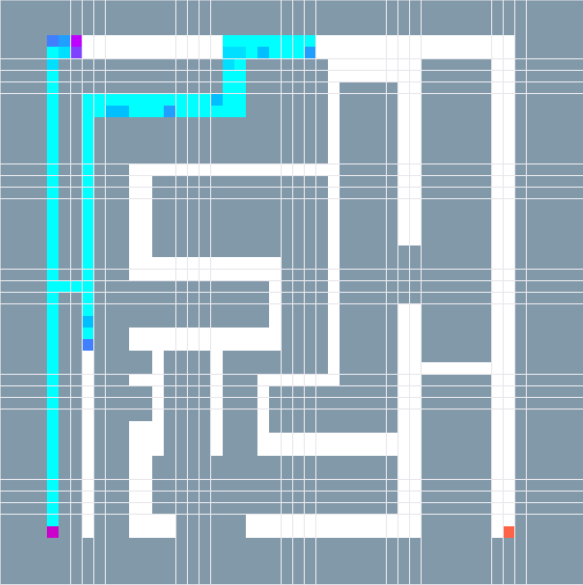
\includegraphics[width=0.32\textwidth]{maze_gpgpu_exp/2_maze_gpgpu}} 
    \subfigure[Tubes creation]{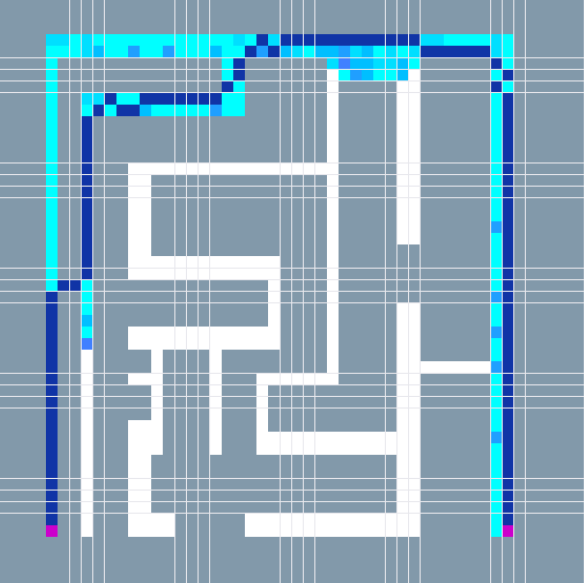
\includegraphics[width=0.32\textwidth]{maze_gpgpu_exp/3_maze_gpgpu}} 
    \subfigure[Simulation end]{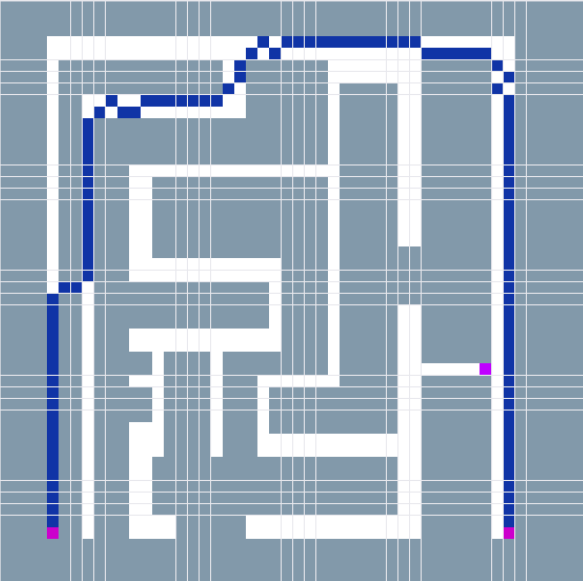
\includegraphics[width=0.32\textwidth]{maze_gpgpu_exp/4_maze_gpgpu}}
    \caption{First maze}
    \label{fig:foobar}
\end{figure}

\paragraph{Second maze}

\begin{center}
 \begin{tabular}{||c c||} 
 \hline
 Parameter & Value \\ [0.5ex] 
 \hline\hline
 GridSize & $50 \times 50$ \\ 
 \hline
 PM & 10000 \\ 
 \hline
 CHA & 100 \\ 
 \hline
 CON & 0.95 \\ 
 \hline
 CAP1 & 0.05 \\ 
 \hline
 CAP2 & 0.01 \\ 
 \hline
 MinAgeDryOut & 1000 \\
 \hline
 ThPM & 20 \\ [1ex] 
 \hline
 \end{tabular}
\end{center}

\begin{figure}[H]
    \centering
    \subfigure[Expansion process]{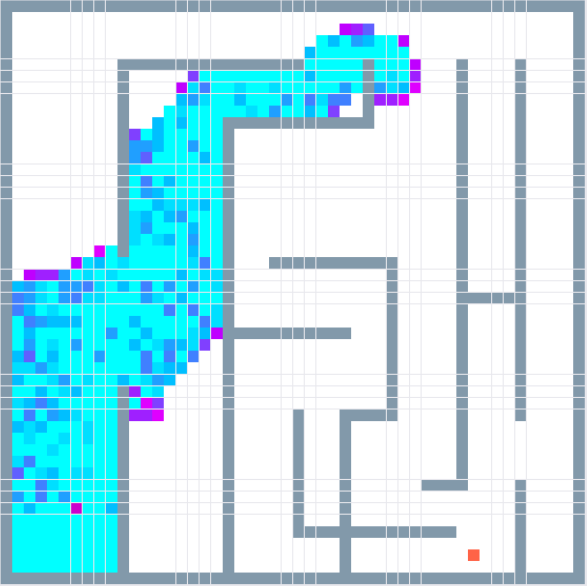
\includegraphics[width=0.32\textwidth]{generic_maze_exp/2_generic_maze}} 
    \subfigure[Tubes creation and shrinking process]{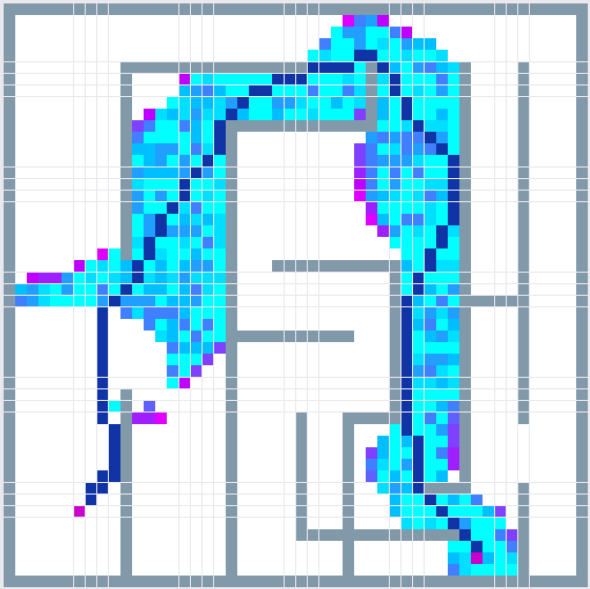
\includegraphics[width=0.32\textwidth]{generic_maze_exp/3_generic_maze}} 
    \subfigure[Simulation end]{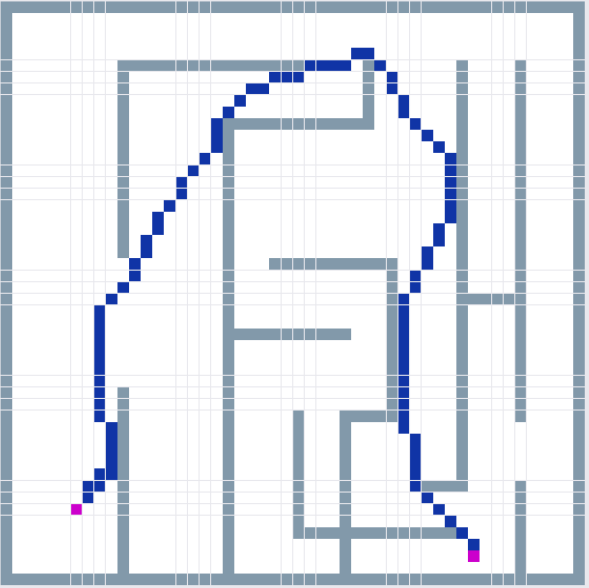
\includegraphics[width=0.32\textwidth]{generic_maze_exp/4_generic_maze}}
    \caption{Second maze}
    \label{fig:foobar}
\end{figure}


\chapter{Analysis of the results}
\section{Network formation}
\label{network_formation}

When running both the simulations the ideal result should be a Minimum Spanning Tree (MST), where there are no cycles and each vertex is connected by the shortest possible path, optimizing all the paths that start from SP considered as root of the MST.
While it's very straightfoward to use a global algorithm to calculate and draw the MST, both the simulations run using only local rules (respecting the definition of CA) and the cells' individual behaviour creates paths that are not always the best. The result for both the CAs is always a spanning tree nonetheless, although never a minimum one.

\par
The results of the two simulations are compared with one of the correct MST for two different network maps in figure~\ref{fig:mst_20_40}.

\begin{figure}[H]
    \centering
    \subfigure[MST of network with 20 nodes]{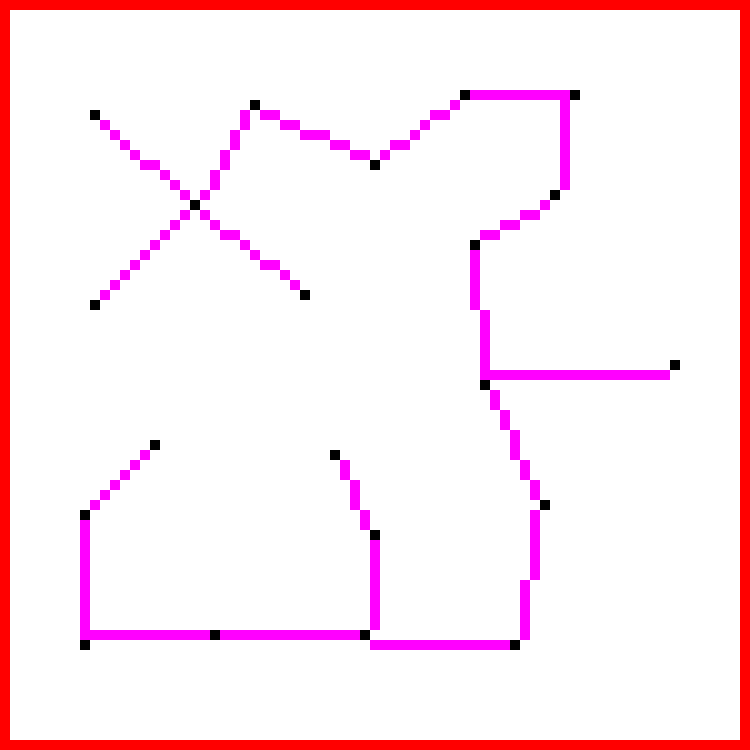
\includegraphics[width=0.40\textwidth]{mst_20}} 
    \subfigure[Experimental result of simulation network with 20 nodes]{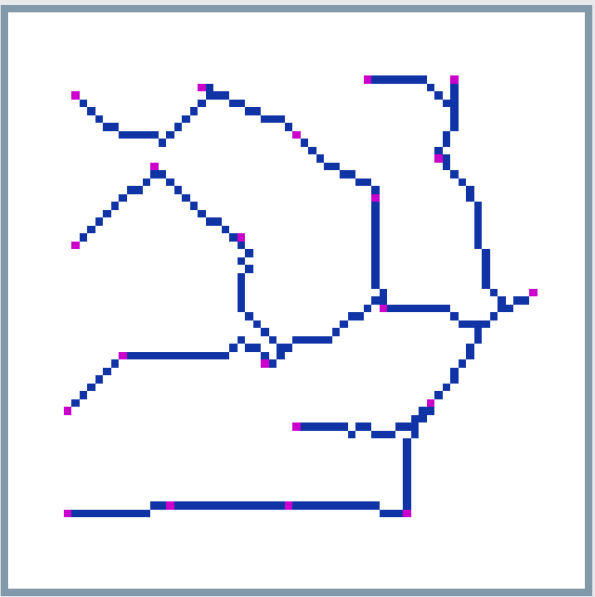
\includegraphics[width=0.40\textwidth]{wsn_20_exp/4_wsn_20}} 
    \subfigure[MST of network with 40 nodes]{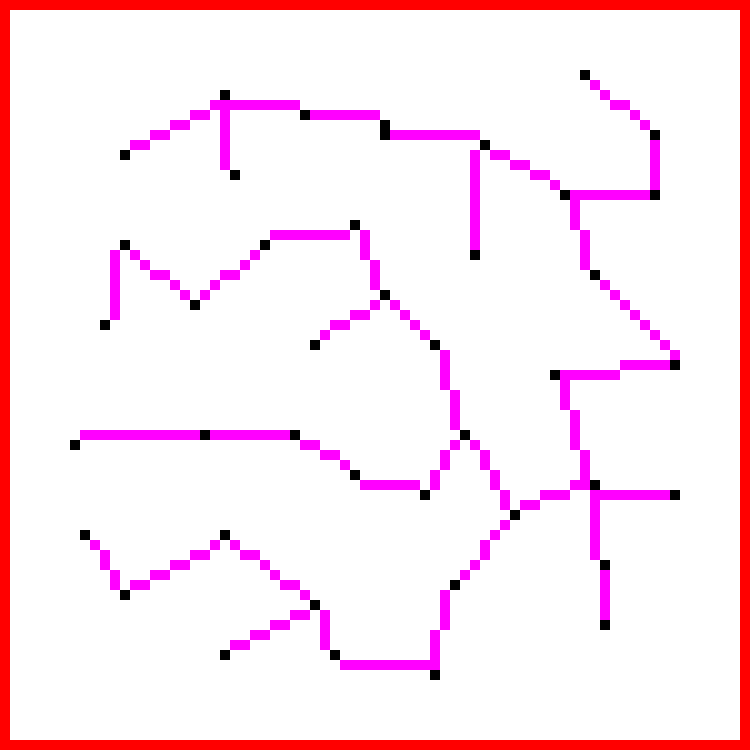
\includegraphics[width=0.40\textwidth]{mst_40}} 
    \subfigure[Experimental result of simulation network with 40 nodes]{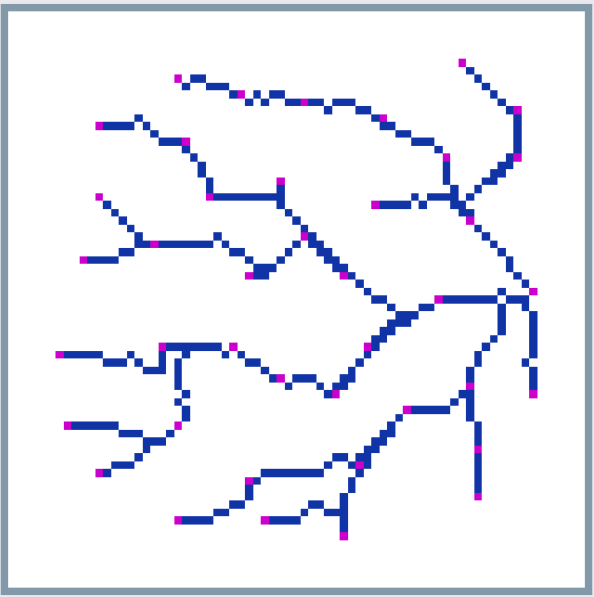
\includegraphics[width=0.40\textwidth]{wsn_40_exp/4_wsn_40}} 
    \caption{MSTs and results simulation comparison for network formation}
    \label{fig:mst_20_40}
\end{figure}

\par
First of all, we need to remember that several valid MSTs can exist for each graph depending on the order of the choices and this is one reason why some archs of the MST are different compared to the results of the simulations.

\par
The diffusion of the $PM$ to the neighbour cells following approximated rules (less accurate than the real Physarum physics) makes the gradient divert from the optimal shortest paths.
Finally another reason why the results differ from the MST is parallelism: any standard MST algorithm searches sequentially the nearest node to add it to the tree, while CAs expand in different locations at the same time because every cell is indipendent from the others. This difference makes some nodes easier to reach even if they are not the nearest from a MST point of view.

\par
For most of the time, the experimental simulation produces archs that are more similar to the MST respect to the paper simulation. For each map a better tuning of the parameters could be made to minimize this error but in all our tests our simulation outperforms the other one.

\par
From laboratory observations, when the Physarum produces his network tubes it's pretty common that two or more tubes share a part to minimize the needed mass, as can be seen in figure~\ref{fig:tube_intersection_red}.

\begin{figure}[H]
  \centering
    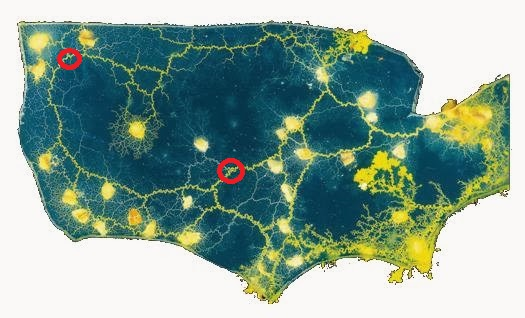
\includegraphics[width=0.48\textwidth]{tube_intersection_red}%
    
  \caption{Tubes intersection in real Physarum}
  \label{fig:tube_intersection_red}
\end{figure}

\par
The paper simulation has never showed this behaviour, creating always clean and completely separated tubes for each different couple of nodes. On the other side, the experimental simulation often produces this kind of interconnected tubes as showed in figure~\ref{fig:wsn_40_red_intersection}.

\begin{figure}[H]
  \centering
    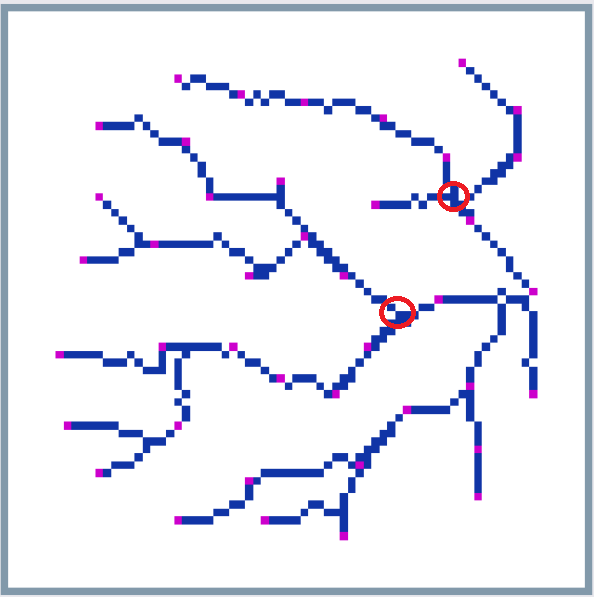
\includegraphics[width=0.48\textwidth]{wsn_40_red_intersection}%
    
  \caption{Tubes intersection in simulated Physarum}
  \label{fig:wsn_40_red_intersection}
\end{figure}

\par
The paper simulation creates his network leaving the map flooded with mould mass everywhere (as seen in figures of section \nameref{network_formation_5}), while our algorithm pushes the dispersed mass towards the tubes, leaving only the network visible as the real Physarum does. For enough large maps with NSs too far from SP, the paper algorithm crashes: as it doesn't respect the mass conservation, some cells reach a mass value so high that it overflows. A solution could be creating a limit value for the mass but in this case a lot of cells (firstly the ones near the margins of the map) would all reach the same limit value, destroying the gradient needed for connecting the NSs with SP.
If our experimental algorithm cannot reach too far NSs, the solution is to simply increase the inizial mould mass so it will be able to expand further. This makes the algorithm very robust and has never crashed during the simulations.

\par
For all these reasons, our experimental model can be considered much more solid and more similar to Physarum's real dynamics, even if we would need more laboratory pictures of all the topologies that the mould can create for a better validation process.

\section{Maze solving}

Maze solving finding the shortest path among all the possibilities is another task in which Physarum always successes. The computer simulations should also be able to solve this task in a very similar manner.

\par
In \cite{Tsompanas2016} the authors explicity say that their updated version of the algorithm is also able to solve mazes without showing any proof of that. Implementing their mathematical equations and the mould behaviour didn't get the results we were looking for: their model cannot solve mazes, even with very high PM value because of similar problems described in \nameref{network_formation}, like loosing the mass gradient when reaching the objective.

\par
We implemented two standard and famous mazes used as examples in Physarum scientific documentation and only the experimental model was able to solve them. The failed attempts of the paper simulation are shown in figures of section \nameref{maze_solving} (subsection \nameref{paper_model}).
Giving enough mass to the mould, the experimental model was able to find the shortest path in every maze as shown in \nameref{maze_solving} (subsection \nameref{experimental_model}), reaching the optimal solution every single time.

\par
If we don't strictly consider the possible routes inside the maze but instead the single cells of the map then the simulation often returns a suboptimal solution with an epsilon error respect to the absolute shortest path as can be seen in figure~\ref{fig:mst_tube}.

\begin{figure}[H]
    \centering
    \subfigure[MST of second maze]{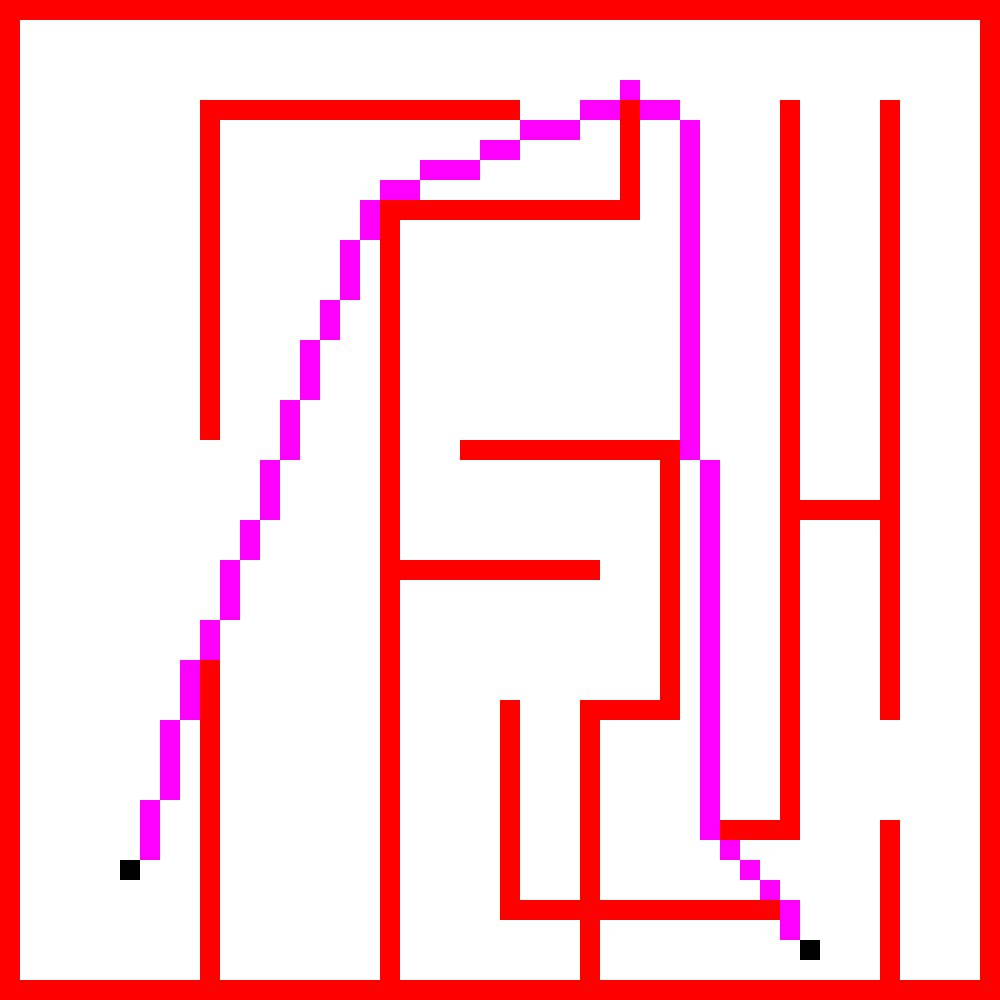
\includegraphics[width=0.40\textwidth]{mst_tube}} 
    \subfigure[Experimental result of second maze]{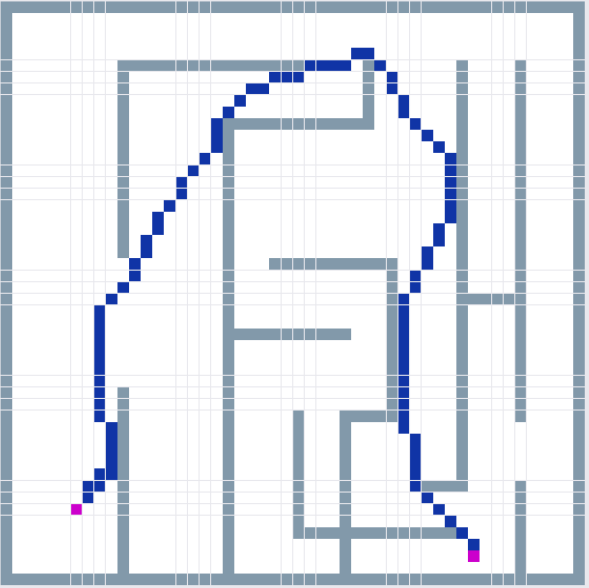
\includegraphics[width=0.40\textwidth]{generic_maze_exp/4_generic_maze}} 
    \caption{MST and result simulation comparison for maze solving}
    \label{fig:mst_tube}
\end{figure}

\par
The cause is the distribution of mass in cells instead of a continuos space: the gradient used to draw the tube is pseudorandomly moved to the pixels near the optimal solution, in a similar fashion to the network archs in section \nameref{network_formation}.

\par
Both the real mould and our experimental model reach the target in the maze with the best possible path, leaving no other useless mass around the map, therefore our CA is validated also for this task.


\chapter{Conclusions}
In this project we presented Physarum polycephalum from a biological point of view and explained complex patterns observed in this puzzling organism. For our purposes of modeling we introduced and defined the Cellular Automata mathematical model  which can perfectly describe slime mould's distributed control because of its properties.

\par
After reviewed the literature on several models, we have decided to use the CA based model of Tsompanas et al. \cite{Tsompanas2016} that mimics the foraging strategy and tubular network formation. In particular, the model is based on the representation of diffusion of chemical attractants by NSs and the attraction of the plasmodium, which initiates its exploration from the starting point (SP), by these chemicals. 

\par
However this model seemed not to follow the true behavior of slime mould and for this reason we have proposed our experimental model - based on this well-known work - which objective was to fix the issues that emerged from the many executions of the original model.

\par
In particular, their algorithm reached the results for the different types of simulation neglecting important realistic constraints. We found their CA's behaviour an excessive approximation of the real mould dynamics, therefore we worked on improving their original algorithm to the point of changing most of the steps.

%TODO
Aggiungere nelle conclusioni la parte dei capitoli 4, 5, 6

%TODO:
Altri sviluppi futuri: REVERSE DRY OUT per renderla più simile al comportamento reale della muffa?

\section{Future developments}
We have drawn a map with two SPs to see the behavior. However, the model is based on a single Physarum at the initial state and therefore uses a single gradient for the creation of the tubes. Therefore it is normal that with two SPs the computation is not successful in these circumstances.

\par
The models based on single Physarum as those cited in the previous chapter addressed only attraction force of just one Physarum towards a food resource.

\par
So a plausible future development concerns the possibility of considering a Physarum competitive behaviour where a group of Physarum with different masses and motivation - hunger and satiety - each having autonomous behaviours react to each other and their own local environment. 

\par
This type of model has already been proposed \cite{hex_phy} and it considered other forces acting on Physarum based on metaheuristics inspired from Physarum behaviour in a competition. They assume that competing Physarum will exert repulsion forces on each other which will affect the evolution of the whole system and so they created a new formula to compute two forces acting on Physarum: 

\begin{itemize}
	\item the chemo attraction force based on the combination of chemical mass and chemical quality
	\item the repulsion negative forces that competing Physarum exert on each other
\end{itemize}

Chemo attraction forces exerted on Physarum will be a function of food resource (with different mass and quality) and Physarum hunger motivation. If Physarum is satisfied, it would appreciate the quality of chemical rather than the mass, and if it is hungry, vice versa.




\bibliographystyle{unsrt}
\bibliography{bibliography}

\end{document}
